\documentclass{beamer}\usepackage[]{graphicx}\usepackage[]{color}
%% maxwidth is the original width if it is less than linewidth
%% otherwise use linewidth (to make sure the graphics do not exceed the margin)
\makeatletter
\def\maxwidth{ %
  \ifdim\Gin@nat@width>\linewidth
    \linewidth
  \else
    \Gin@nat@width
  \fi
}
\makeatother

\definecolor{fgcolor}{rgb}{0.345, 0.345, 0.345}
\newcommand{\hlnum}[1]{\textcolor[rgb]{0.686,0.059,0.569}{#1}}%
\newcommand{\hlstr}[1]{\textcolor[rgb]{0.192,0.494,0.8}{#1}}%
\newcommand{\hlcom}[1]{\textcolor[rgb]{0.678,0.584,0.686}{\textit{#1}}}%
\newcommand{\hlopt}[1]{\textcolor[rgb]{0,0,0}{#1}}%
\newcommand{\hlstd}[1]{\textcolor[rgb]{0.345,0.345,0.345}{#1}}%
\newcommand{\hlkwa}[1]{\textcolor[rgb]{0.161,0.373,0.58}{\textbf{#1}}}%
\newcommand{\hlkwb}[1]{\textcolor[rgb]{0.69,0.353,0.396}{#1}}%
\newcommand{\hlkwc}[1]{\textcolor[rgb]{0.333,0.667,0.333}{#1}}%
\newcommand{\hlkwd}[1]{\textcolor[rgb]{0.737,0.353,0.396}{\textbf{#1}}}%

\usepackage{framed}
\makeatletter
\newenvironment{kframe}{%
 \def\at@end@of@kframe{}%
 \ifinner\ifhmode%
  \def\at@end@of@kframe{\end{minipage}}%
  \begin{minipage}{\columnwidth}%
 \fi\fi%
 \def\FrameCommand##1{\hskip\@totalleftmargin \hskip-\fboxsep
 \colorbox{shadecolor}{##1}\hskip-\fboxsep
     % There is no \\@totalrightmargin, so:
     \hskip-\linewidth \hskip-\@totalleftmargin \hskip\columnwidth}%
 \MakeFramed {\advance\hsize-\width
   \@totalleftmargin\z@ \linewidth\hsize
   \@setminipage}}%
 {\par\unskip\endMakeFramed%
 \at@end@of@kframe}
\makeatother

\definecolor{shadecolor}{rgb}{.97, .97, .97}
\definecolor{messagecolor}{rgb}{0, 0, 0}
\definecolor{warningcolor}{rgb}{1, 0, 1}
\definecolor{errorcolor}{rgb}{1, 0, 0}
\newenvironment{knitrout}{}{} % an empty environment to be redefined in TeX

\usepackage{alltt}
\usefonttheme[onlymath]{serif}

\usepackage[portuguese]{babel}
\usepackage{graphicx}
\usepackage{ulem} % Para texto em strikeout
\usepackage{amsmath}
\usepackage{amssymb}

\usetheme{m}

\ifdefined\knitrout 
\renewenvironment{knitrout}{\setlength{\topsep}{0mm}}{}
\else
\fi

\title{Aula 6: Modelos Lineares Gerais III}
\subtitle{Análise Estatística e Modelagem de Dados Ecológicos}
\author{\textbf{Thiago S. F. Silva} - tsfsilva@rc.unesp.br}
\institute{Programa de Pós Graduação em Ecologia e Biodiversidade - UNESP}
\date{\today}

\graphicspath{{C:/Users/thiago/OneDrive/UNESP/Pos_graduacao/Eco/2015/Estatistica_2015/Aulas/Aula_6_diagnostico_remediacao/figuras/}}
\IfFileExists{upquote.sty}{\usepackage{upquote}}{}
\begin{document}



%===============================================================================%
\begin{frame}[plain] % plain avoids a badbox error from page number in title page
  \titlepage
\end{frame}

\begin{frame}{Outline}
  \tableofcontents
\end{frame}
%===============================================================================%

\section{Diagnóstico, Remediação e Validação}

%===============================================================================%
\begin{frame}{Diagnóstico, Remediação e Validação}

Nossos modelos lineares são baseados em uma série de pressuposições, a lembrar:
\vfill
\begin{enumerate}
  \item Os valores/níveis de $X$ são medidos sem erro \pause
  \vfill
  \item Existe uma relação linear entre $X$ e $Y$ (só para regressão) \pause
  \vfill
  \item Os erros $\varepsilon$ (e por consequência, $Y$) tem variância constante ($\sigma^2$) \pause
  \vfill
  \item Os erros $\varepsilon$ (e por consequência, $Y$) são independentes \pause
  \vfill
  \item Os erros $\varepsilon$ (e por consequência, $Y$) são normalmente distribuídos:
  \vfill
  \begin{itemize}
    \item $\varepsilon \sim N(0,\sigma^2)$
    \vfill
    \item  $Y\sim N(\beta _0 + \beta _1 X,\sigma^2)$
  \end{itemize}
\end{enumerate}


\end{frame}
%===============================================================================%

%===============================================================================%
\begin{frame}{Diagnóstico e Remediação}

Muitas vezes, estas pressuposições não correspondem à realidade. Por esta razão, todo processo de modelagem inclui etapas de diagnóstico, remediação, e validação: \pause
\vfill
\textbf{Diagnóstico}: processo de avaliação da adequação dos dados e resultados às pressuposições do modelo. \pause
\vfill
\textbf{Remediação}: processo de melhoria da adequação dos dados e resultados às pressuposições do modelo. \pause
\vfill
\textbf{Validação}: processo de verificação da performance do modelo na explicação/previsão do fenômeno de interesse

\end{frame}
%===============================================================================%


\section{Análise de resíduos}


% %===============================================================================%
% \begin{frame}{Análise de resíduos}
% 
% A análise descritiva e gráfica dos resíduos do modelo pode diagnosticar a maioria das violações às pressuposições do modelo.
% \vfill
% Em alguns casos, pode ser útil normalizar o valor dos resíduos: \pause
% \vfill
% \textbf{Resíduos Normalizados:} Valores originais normalizados pela variância. \pause
% \vfill
% \textbf{Resíduos Estudantizados:} (\emph{studentized residuals}) Valores originais divididos pela variância dos resíduos da mesma regressão, com o valor em questão excluído. Tem esse nome pois seguem uma distribuição $t$.\pause
% 
% \end{frame}
% %===============================================================================%

%===============================================================================%
\begin{frame}{Análise de resíduos}

\begin{columns}[t]

\column{0.6\linewidth}
\small

Uma das princpais análises diagnósticas é um scatterplot dos resíduos vs.  valores estimados ($\hat Y$) \pause

\bigskip

Vejamos um exemplo de um modelo de regressão apropriado: 
\begin{itemize}
\item Resíduos aletoriamente distribuidos ao redor de zero 
\item Variação constante ao longo de $Y_i$
\end{itemize}

\column{0.4\linewidth}

\begin{knitrout}
\definecolor{shadecolor}{rgb}{0.969, 0.969, 0.969}\color{fgcolor}
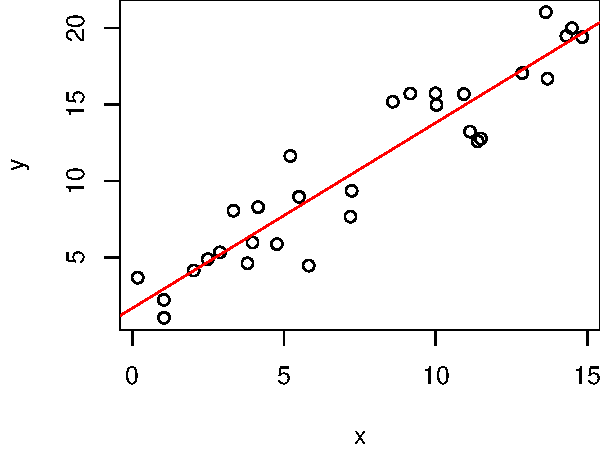
\includegraphics[width=1\linewidth]{figure/reg1-1} 

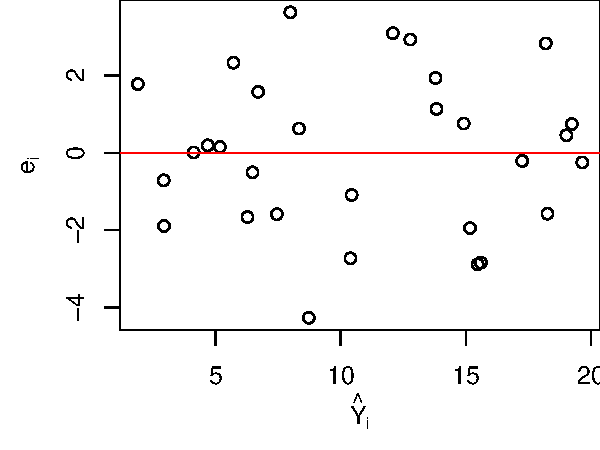
\includegraphics[width=1\linewidth]{figure/reg1-2} 

\end{knitrout}
\end{columns}


\end{frame}
%===============================================================================%


%===============================================================================%
\begin{frame}{Análise de resíduos}

\begin{columns}[c]

\column{0.6\linewidth}
\small

Uma das princpais análises diagnósticas é um scatterplot dos resíduos vs.  valores estimados ($\hat Y$) 

\bigskip

Vejamos um exemplo de um modelo de regressão apropriado:
\begin{itemize}
\item Resíduos aletoriamente distribuidos ao redor de zero
\item Variação constante ao longo de $\hat{Y}_i$
\end{itemize}

\column{0.4\linewidth}

\begin{knitrout}
\definecolor{shadecolor}{rgb}{0.969, 0.969, 0.969}\color{fgcolor}
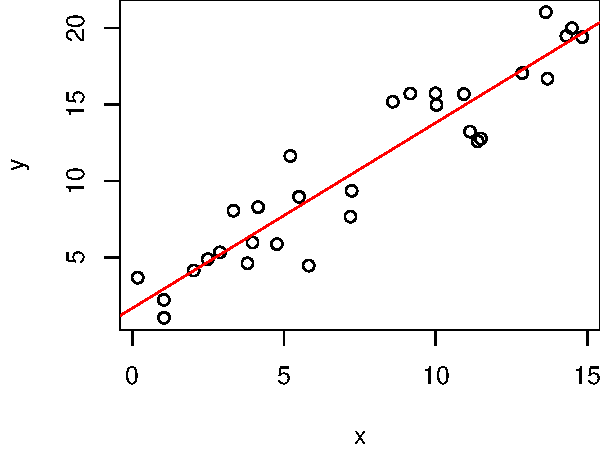
\includegraphics[width=1\linewidth]{figure/r2-1} 

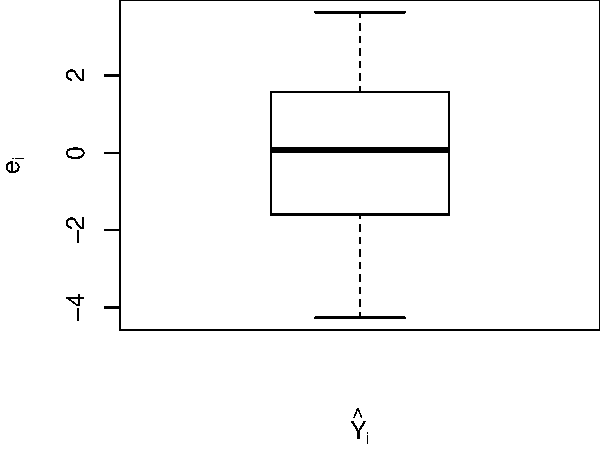
\includegraphics[width=1\linewidth]{figure/r2-2} 

\end{knitrout}
\end{columns}


\end{frame}
%===============================================================================%


%===============================================================================%
\begin{frame}{Análise de resíduos}

\begin{columns}[c]

\column{0.6\linewidth}
\small

Dados com resíduos não-normais: 
\begin{itemize}
\item Resíduos positivos maiores do que resíduos negativos 
\item Distribuição Assimétrica 
\end{itemize}

\column{0.4\linewidth}

\begin{knitrout}
\definecolor{shadecolor}{rgb}{0.969, 0.969, 0.969}\color{fgcolor}
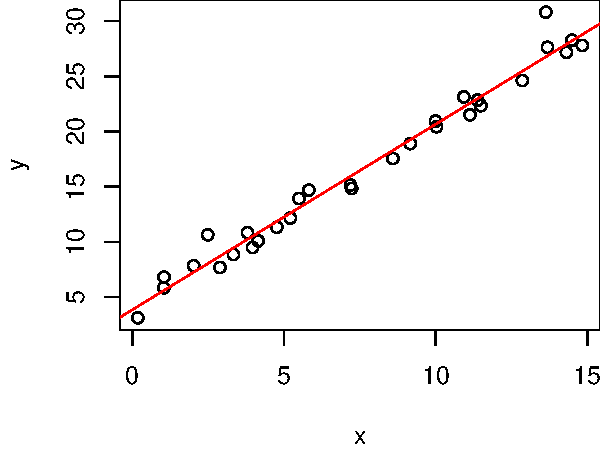
\includegraphics[width=1\linewidth]{figure/r3-1} 

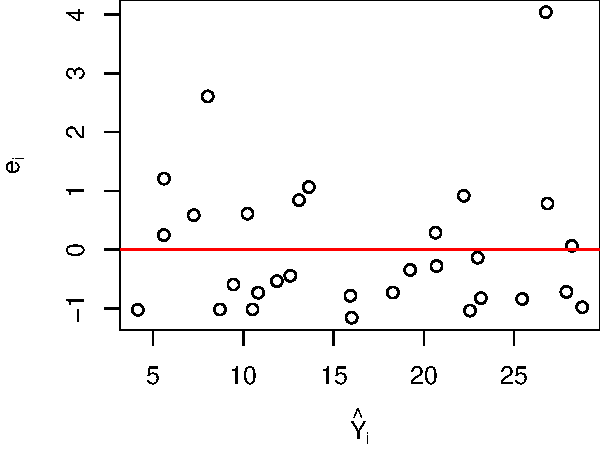
\includegraphics[width=1\linewidth]{figure/r3-2} 

\end{knitrout}
\end{columns}

\end{frame}
%===============================================================================%

%===============================================================================%
\begin{frame}{Análise de resíduos}

\begin{columns}[c]

\column{0.6\linewidth}
\small

Dados com resíduos não-normais: 
\begin{itemize}
\item Resíduos positivos maiores do que resíduos negativos 
\item Distribuição Assimétrica 
\end{itemize}

\column{0.4\linewidth}

\begin{knitrout}
\definecolor{shadecolor}{rgb}{0.969, 0.969, 0.969}\color{fgcolor}
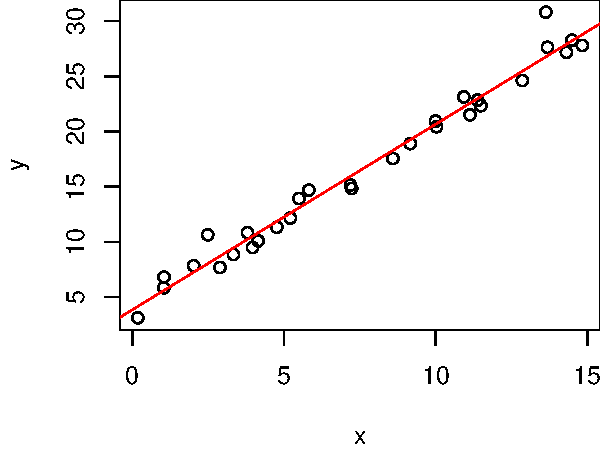
\includegraphics[width=1\linewidth]{figure/r4-1} 

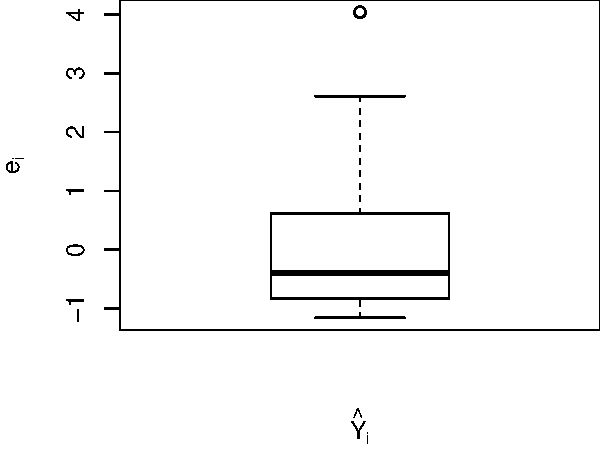
\includegraphics[width=1\linewidth]{figure/r4-2} 

\end{knitrout}
\end{columns}

\end{frame}
%===============================================================================%


%===============================================================================%
\begin{frame}{Análise de resíduos}

\begin{columns}[c]

\column{0.6\linewidth}
\small

Resíduos não-normais: \textbf{Q-Q plot}
\begin{itemize}
\item Ferramenta gráfica bastante utilizada para avaliação de aderência à normalidade \pause
\item Plota os quantis dos dados contra os quantis correspondentes de uma distribuição normal com os mesmos parâmetros: $N(0, s^2)$ \pause
\item Quanto mais normal a distribuição, mais ``iguais'' serão os quantis \pause
\end{itemize}

\column{0.4\linewidth}

\begin{knitrout}
\definecolor{shadecolor}{rgb}{0.969, 0.969, 0.969}\color{fgcolor}
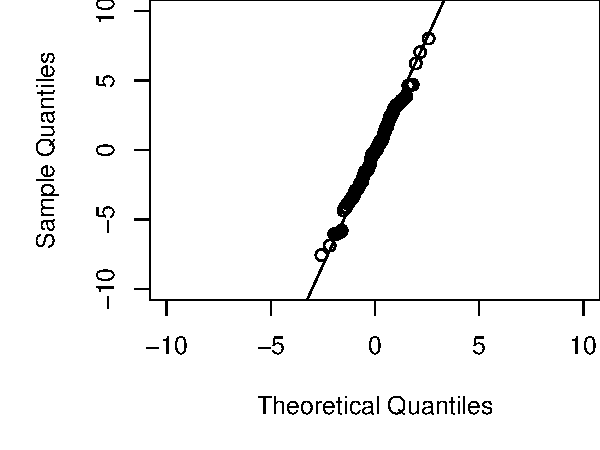
\includegraphics[width=1\linewidth]{figure/r5-1} 

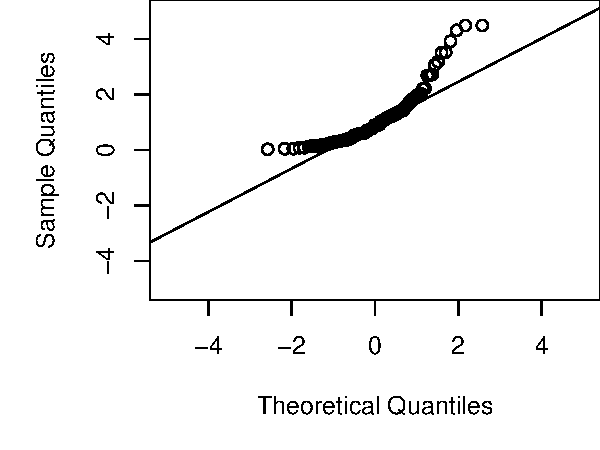
\includegraphics[width=1\linewidth]{figure/r5-2} 

\end{knitrout}
\end{columns}

\end{frame}
%===============================================================================%


%===============================================================================%
\begin{frame}{Análise de resíduos}

\begin{columns}[c]

\column{0.6\linewidth}

\small{Dados com resíduos heteroscedásticos:} \pause

\begin{itemize}
\begin{scriptsize}


\item \textbf{homoscedástico} = variância constante

\item \textbf{heteroscedástico} = variância inconstante \pause

\end{scriptsize}

\item Resíduos aleatoriamente distribuídos ao redor de zero 

\item Variância dos resíduos aumenta (ou diminui) ao longo de $\hat Y$ 

\end{itemize}

\column{0.4\linewidth}

\begin{knitrout}
\definecolor{shadecolor}{rgb}{0.969, 0.969, 0.969}\color{fgcolor}
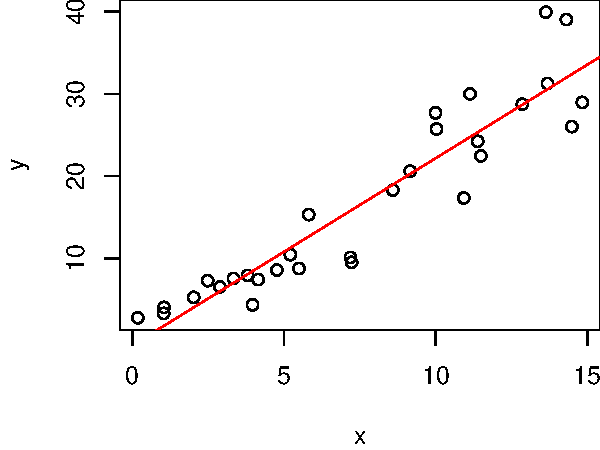
\includegraphics[width=1\linewidth]{figure/r6-1} 

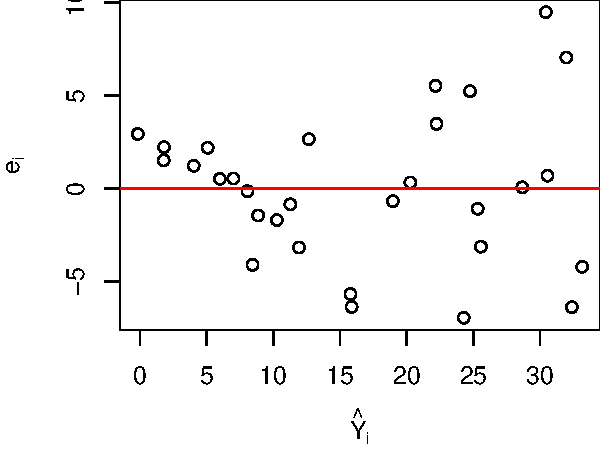
\includegraphics[width=1\linewidth]{figure/r6-2} 

\end{knitrout}
\end{columns}

\end{frame}
%===============================================================================%

%===============================================================================%
\begin{frame}{Análise de resíduos}

\begin{columns}[c]

\column{0.6\linewidth}
\small{Dados com resíduos heteroscedásticos:} \pause

\begin{itemize}

\begin{scriptsize}

\item \textbf{homoscedástico} = variância constante

\item \textbf{heteroscedástico} = variância inconstante 

\end{scriptsize}

\item Resíduos aleatoriamente distribuídos ao redor de zero 

\item Variância dos resíduos aumenta (ou diminui) ao longo de $\hat Y$ 

\end{itemize}

\column{0.4\linewidth}

\begin{knitrout}
\definecolor{shadecolor}{rgb}{0.969, 0.969, 0.969}\color{fgcolor}
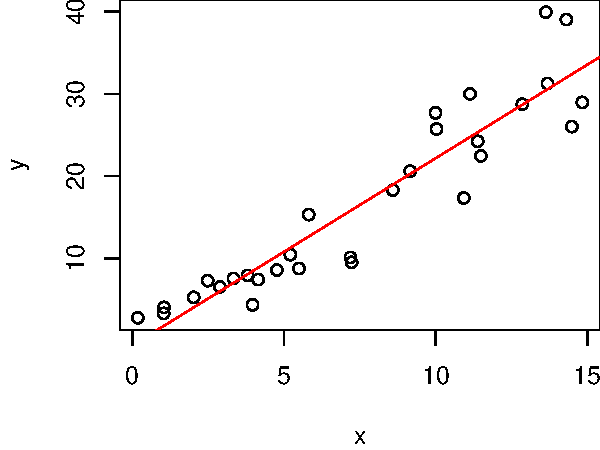
\includegraphics[width=1\linewidth]{figure/r7-1} 

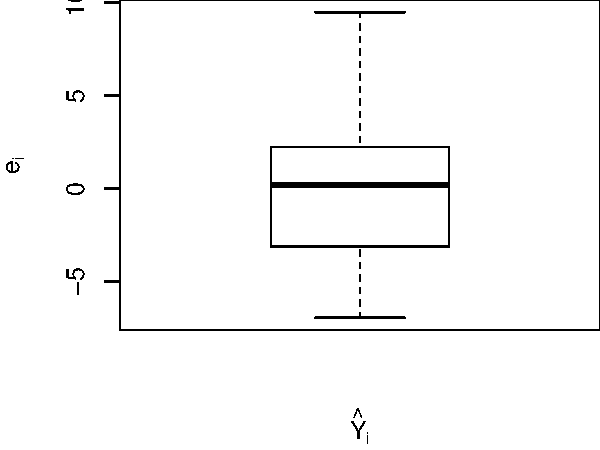
\includegraphics[width=1\linewidth]{figure/r7-2} 

\end{knitrout}
\end{columns}

\end{frame}
%============================================================================%




%===============================================================================%
\begin{frame}{Análise de resíduos}

\begin{columns}[c]

\column{0.6\linewidth}
\small

Dados com resíduos não-independentes:

\bigskip
\textbf{Curva de Keeling }\pause

Concentração de CO2 atmosférico medido em Mauna Loa, Hawaii
\bigskip
\begin{itemize}
\item Resíduos distribuidos sistematicamente ao redor de zero
\end{itemize}

\column{0.4\linewidth}

\begin{knitrout}
\definecolor{shadecolor}{rgb}{0.969, 0.969, 0.969}\color{fgcolor}
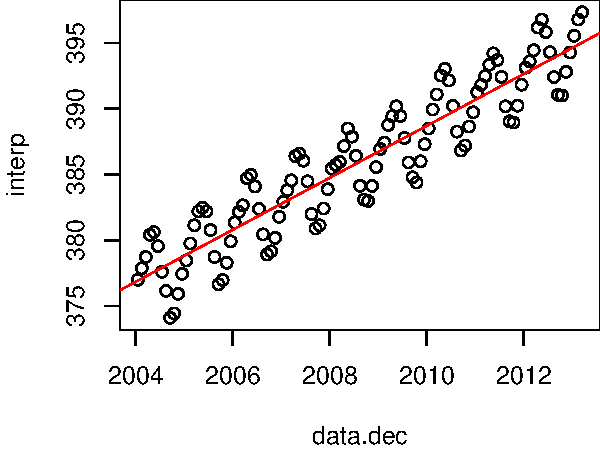
\includegraphics[width=1\linewidth]{figure/r8-1} 

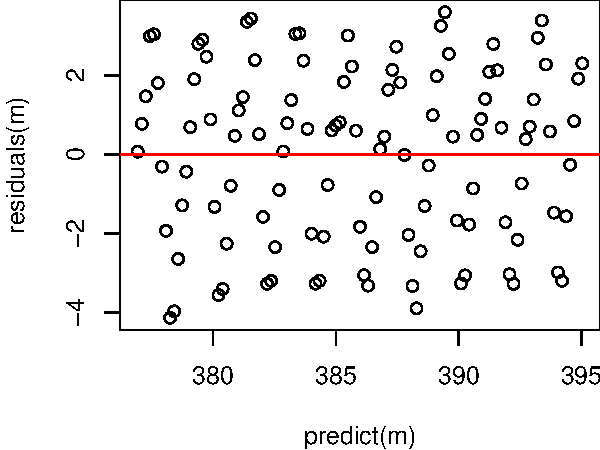
\includegraphics[width=1\linewidth]{figure/r8-2} 

\end{knitrout}
\end{columns}

\end{frame}
%============================================================================%

%===============================================================================%
\begin{frame}{Análise de resíduos}

\begin{columns}[c]

\column{0.6\linewidth}
\small

Dados com resíduos não-independentes:

\bigskip
\textbf{Curva de Keeling }

Concentração de CO2 atmosférico medido em Mauna Loa, Hawaii
\bigskip
\begin{itemize}
\item Resíduos distribuídos sistematicamente ao redor de zero
\end{itemize}


\column{0.4\linewidth}

\begin{knitrout}
\definecolor{shadecolor}{rgb}{0.969, 0.969, 0.969}\color{fgcolor}
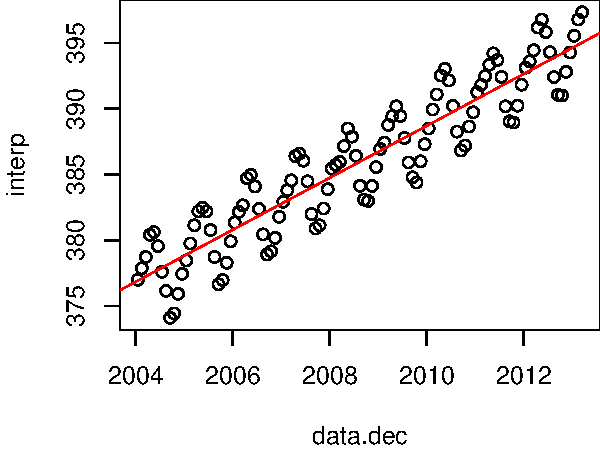
\includegraphics[width=1\linewidth]{figure/r9-1} 

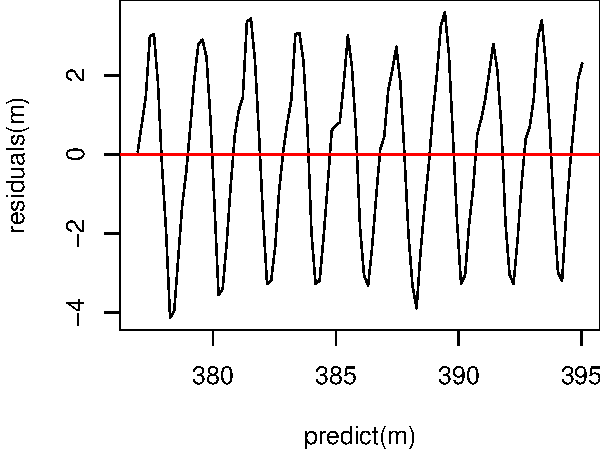
\includegraphics[width=1\linewidth]{figure/r9-2} 

\end{knitrout}
\end{columns}

\end{frame}
%============================================================================%

%===============================================================================%
\begin{frame}{Análise de resíduos}

\begin{columns}[c]

\column{0.6\linewidth}
\small


Dados com resíduos não-independentes:

\bigskip
\textbf{Curva de Keeling }

Concetração de CO2 atmosférico medido em Mauna Loa, Hawaii
\bigskip
\begin{itemize}
\item Resíduos distribuidos sistematicamente ao redor de zero
\end{itemize}
\column{0.4\linewidth}

\begin{knitrout}
\definecolor{shadecolor}{rgb}{0.969, 0.969, 0.969}\color{fgcolor}
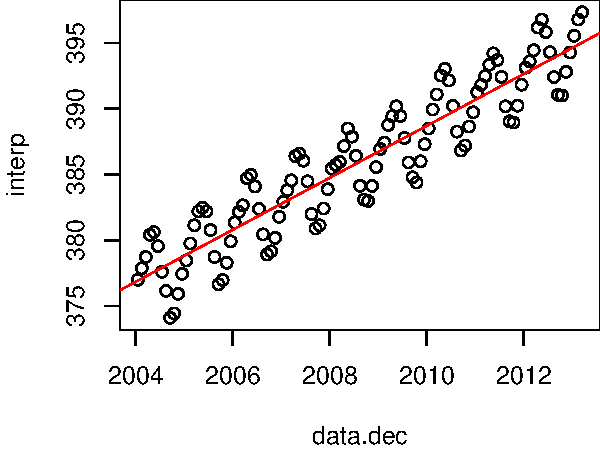
\includegraphics[width=1\linewidth]{figure/r10-1} 

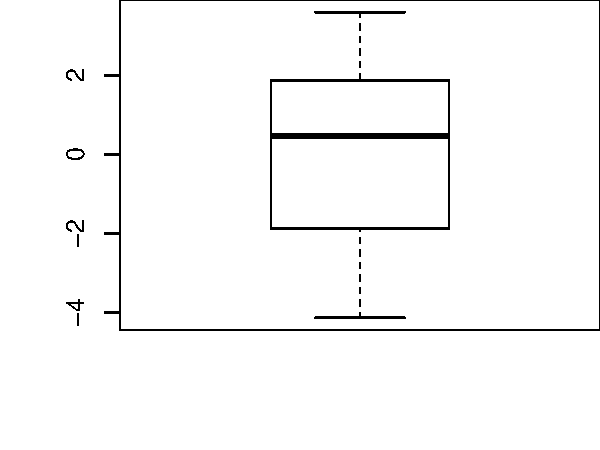
\includegraphics[width=1\linewidth]{figure/r10-2} 

\end{knitrout}
\end{columns}

\end{frame}
%============================================================================%


%===============================================================================%
\begin{frame}{Análise de resíduos}

\begin{columns}[c]

\column{0.6\linewidth}
\small


\textbf{Função de Autocorrelação}

\bigskip
Plota a correlação entre $X$ e seus próprios valores, com diferentes lags.

\column{0.4\linewidth}

\begin{knitrout}
\definecolor{shadecolor}{rgb}{0.969, 0.969, 0.969}\color{fgcolor}
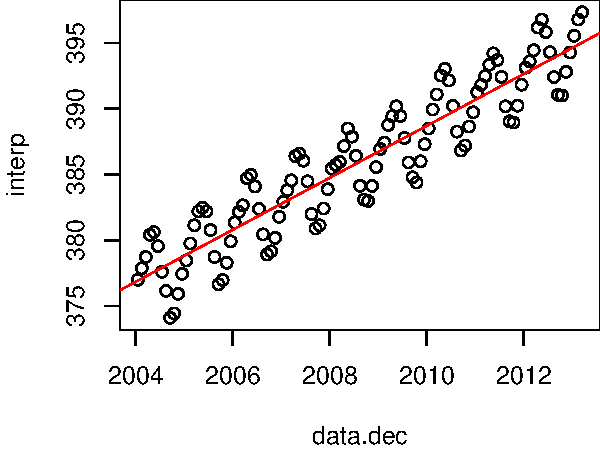
\includegraphics[width=1\linewidth]{figure/r101-1} 

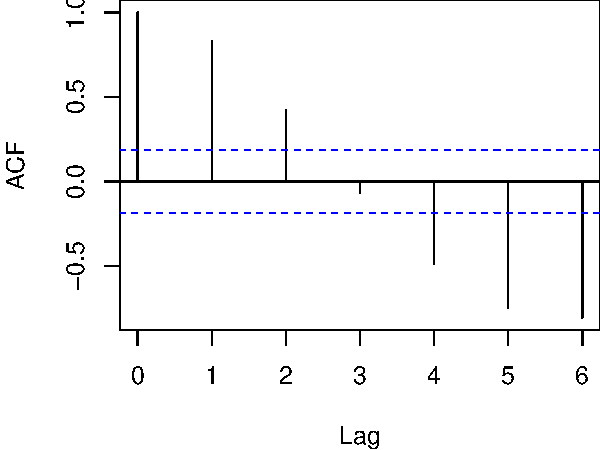
\includegraphics[width=1\linewidth]{figure/r101-2} 

\end{knitrout}
\end{columns}

\end{frame}
%============================================================================%



%===============================================================================%
\begin{frame}{Análise de resíduos}

\begin{columns}[c]

\column{0.6\linewidth}
\small


Relação entre $X$ e $Y$ não é linear \pause

\bigskip
\begin{itemize}
\item Resíduos distribuidos segundo um padrão
\item O padrão sugere o tipo de relação
\end{itemize}

\column{0.4\linewidth}

\begin{knitrout}
\definecolor{shadecolor}{rgb}{0.969, 0.969, 0.969}\color{fgcolor}
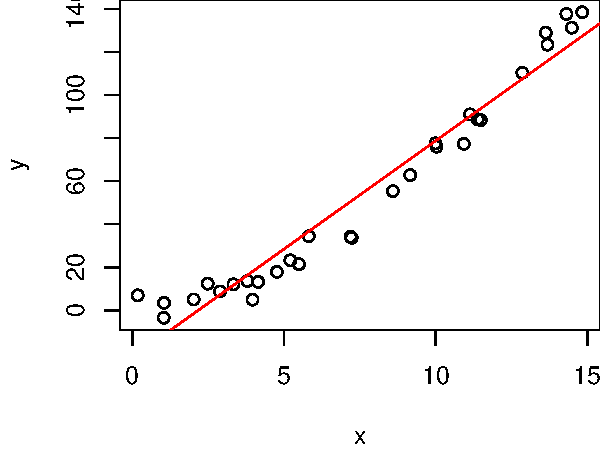
\includegraphics[width=1\linewidth]{figure/r11-1} 

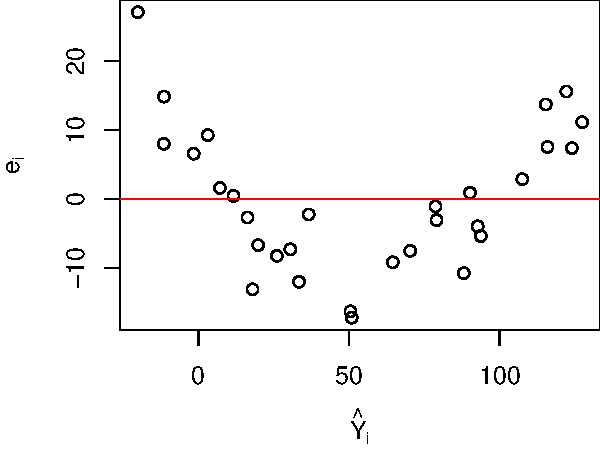
\includegraphics[width=1\linewidth]{figure/r11-2} 

\end{knitrout}
\end{columns}

\end{frame}
%============================================================================%


%===============================================================================%
\begin{frame}{Análise de resíduos}

\begin{columns}[c]

\column{0.6\linewidth}
\small


Relação entre $X$ e $Y$ não é linear

\bigskip
\begin{itemize}
\item Resíduos distribuidos segundo um padrão
\item O padrão sugere o tipo de relação
\end{itemize}

\column{0.4\linewidth}

\begin{knitrout}
\definecolor{shadecolor}{rgb}{0.969, 0.969, 0.969}\color{fgcolor}
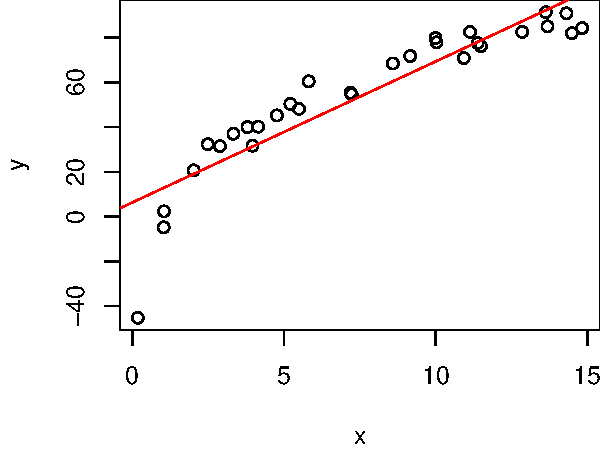
\includegraphics[width=1\linewidth]{figure/r12-1} 

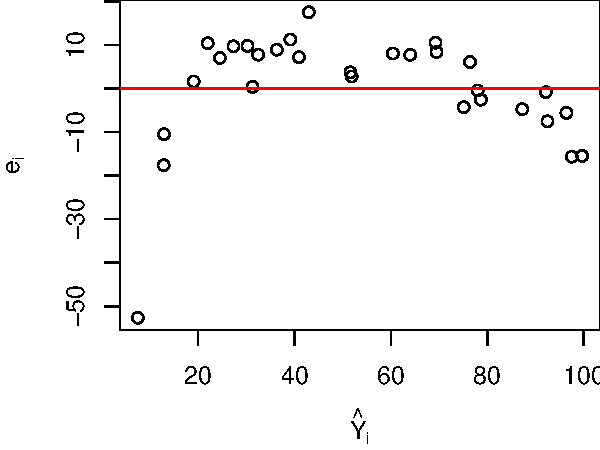
\includegraphics[width=1\linewidth]{figure/r12-2} 

\end{knitrout}
\end{columns}

\end{frame}
%============================================================================%



%===============================================================================%
\begin{frame}{Análise de resíduos}

\begin{columns}[c]

\column{0.6\linewidth}
\small


Ausência de uma variável explicativa

\bigskip
\begin{itemize}
\item Grande parte da variância não explicada por $X_1$ 
\item Resíduos nem sempre revelam um padrão
\item Mas pode ocorrer forte relação entre os resíduos e a varável omitida
\end{itemize}

\column{0.4\linewidth}

\begin{knitrout}
\definecolor{shadecolor}{rgb}{0.969, 0.969, 0.969}\color{fgcolor}
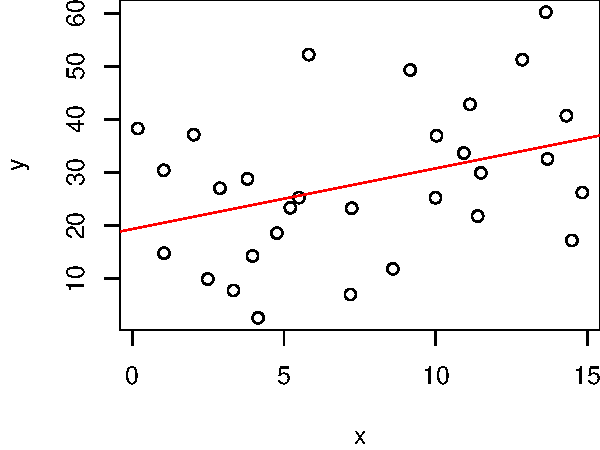
\includegraphics[width=1\linewidth]{figure/r13-1} 

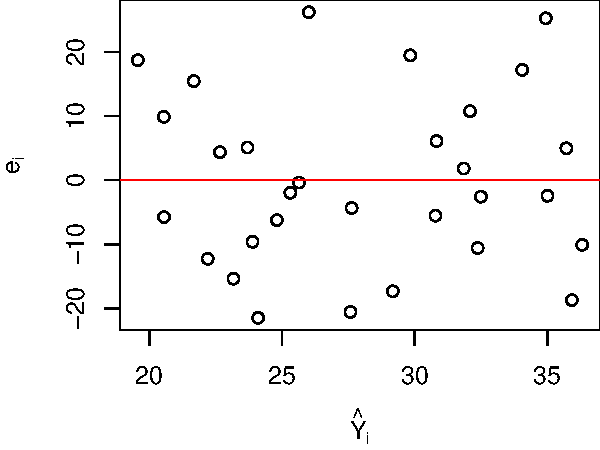
\includegraphics[width=1\linewidth]{figure/r13-2} 

\end{knitrout}
\end{columns}

\end{frame}
%============================================================================%

%===============================================================================%
\begin{frame}{Análise de resíduos}

\begin{columns}[c]

\column{0.6\linewidth}
\small


Ausência de uma variável explicativa

\bigskip
\begin{itemize}
\item Grande parte da variância não explicada por $X_1$ 
\item Resíduos nem sempre revelam um padrão
\item Mas pode ocorrer forte relação entre os resíduos e a varável omitida
\end{itemize}

\column{0.4\linewidth}

\begin{knitrout}
\definecolor{shadecolor}{rgb}{0.969, 0.969, 0.969}\color{fgcolor}
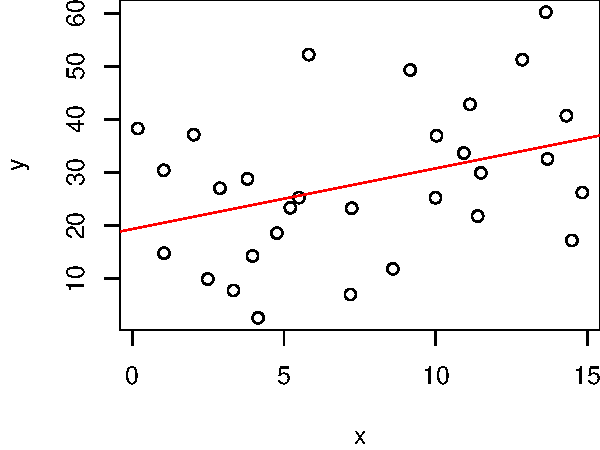
\includegraphics[width=1\linewidth]{figure/r14-1} 

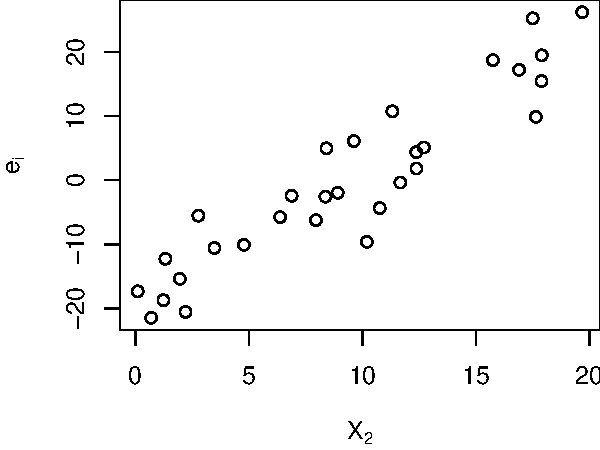
\includegraphics[width=1\linewidth]{figure/r14-2} 

\end{knitrout}
\end{columns}

\end{frame}
%============================================================================%

%===============================================================================%
\begin{frame}{Tipos de Resíduos}
\footnotesize

\textbf{Resíduos Brutos (\emph{Raw})}: Os resíduos originais do modelo, na escala de valores original de $Y$. Se oriundos de um modelo múltiplo, podem assumir valores "estranhos".
\vfill
\textbf{Resíduos Normalizados (\emph{Standardized})}: Resíduos originais, divididos pelo erro padrão dos resíduos: $e_i / \sqrt{MQ_{Res}}$. Contudo, apesar da pressuposição de variância constante dos \textbf{erros ($\mathbf{\varepsilon}$)}, os resíduos tendem a ser menos confiáveis quanto mais distante de $(\bar{X},\bar{Y})$.  \pause
\vfill
\textbf{Resíduos Estudantizados (\emph{Studentized})}: Normalização dos resíduos que leva em conta esse efeito de distância de $\bar{X}$, através da fórmula $e_i / MQ_{Res} \times \sqrt{(1 - h_{ii})}$. $h_{ii}$ é um elemento da matriz desenho do modelo, que captura esse efeito.

\end{frame}
%============================================================================%

%===============================================================================%
\begin{frame}{Análise de resíduos}

\begin{columns}[t]

\column{0.6\linewidth}
\small

\begin{itemize}
\item \textbf{Resíduos Brutos} 
\end{itemize}

\column{0.4\linewidth}

\begin{knitrout}
\definecolor{shadecolor}{rgb}{0.969, 0.969, 0.969}\color{fgcolor}
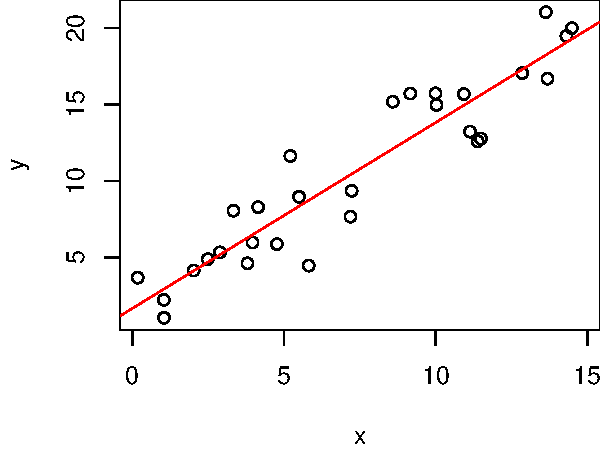
\includegraphics[width=1\linewidth]{figure/rawres-1} 

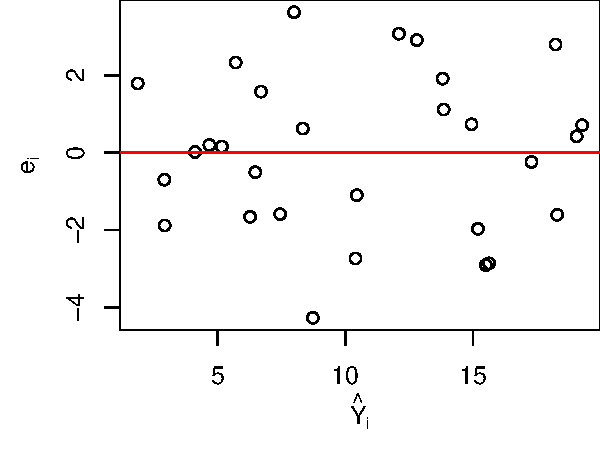
\includegraphics[width=1\linewidth]{figure/rawres-2} 

\end{knitrout}
\end{columns}


\end{frame}
%===============================================================================%

%===============================================================================%
\begin{frame}{Análise de resíduos}

\begin{columns}[t]

\column{0.6\linewidth}
\small

\begin{itemize}
\item Resíduos Brutos
\item \textbf{Resíduos Normalizados}
\end{itemize}

\column{0.4\linewidth}

\begin{knitrout}
\definecolor{shadecolor}{rgb}{0.969, 0.969, 0.969}\color{fgcolor}
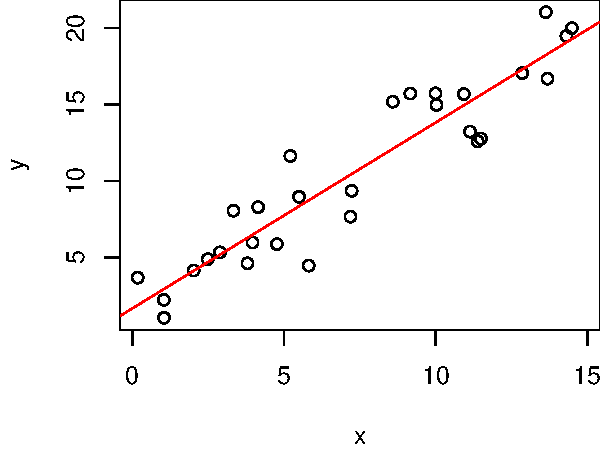
\includegraphics[width=1\linewidth]{figure/stdres-1} 

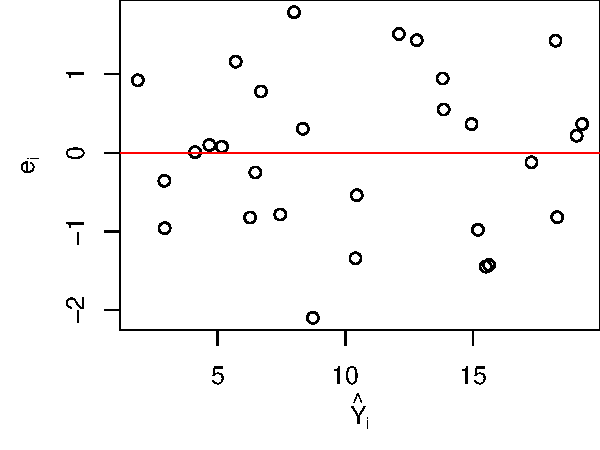
\includegraphics[width=1\linewidth]{figure/stdres-2} 

\end{knitrout}
\end{columns}


\end{frame}
%===============================================================================%


%===============================================================================%
\begin{frame}{Análise de resíduos}

\begin{columns}[t]

\column{0.6\linewidth}
\small

\begin{itemize}
\item Resíduos Brutos
\item Resíduos Normalizados
\item \textbf{Resíduos Estudantizados}
\end{itemize}

\column{0.4\linewidth}

\begin{knitrout}
\definecolor{shadecolor}{rgb}{0.969, 0.969, 0.969}\color{fgcolor}
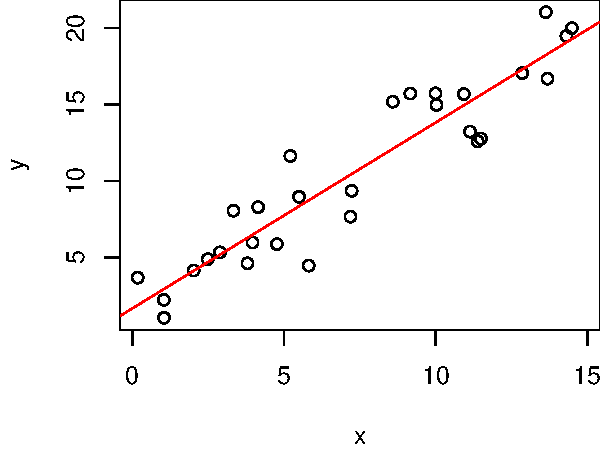
\includegraphics[width=1\linewidth]{figure/studres-1} 

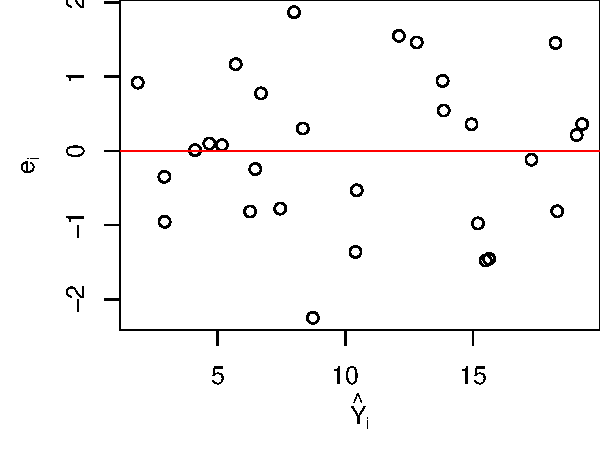
\includegraphics[width=1\linewidth]{figure/studres-2} 

\end{knitrout}
\end{columns}


\end{frame}
%===============================================================================%

%===============================================================================%
\begin{frame}{Pontos Influentes}

Outro diagnóstico importante é a avaliação do efeito de observações isoladas sobre o ajuste final do modelo linear: \pause
\vfill
\textbf{Leverage}: Mede o efeito de valores extremos de $X$. \emph{Leverage} vem de \emph{lever} (alavanca). Valores extremos de $X$ podem alavancar a reta de regressão, que se ``equilibra'' em $(\bar{X},\bar{Y})$ 
\pause
\vfill
\textbf{Distância:} Mede o efeito de valores extremos de $Y$ (resíduos extremos). \pause
\vfill
\textbf{Influência:} Combinação de distância e \emph{leverage}, captura efeito total de um \emph{outlier} sobre a reta de regressão

\end{frame}
%============================================================================%


%===============================================================================%
\begin{frame}{Pontos Influentes}

É possível ter um ponto com \emph{leverage} alto, e influência baixa? \pause
\vfill
\begin{columns}[c]

\column{0.5\linewidth}
\begin{knitrout}
\definecolor{shadecolor}{rgb}{0.969, 0.969, 0.969}\color{fgcolor}
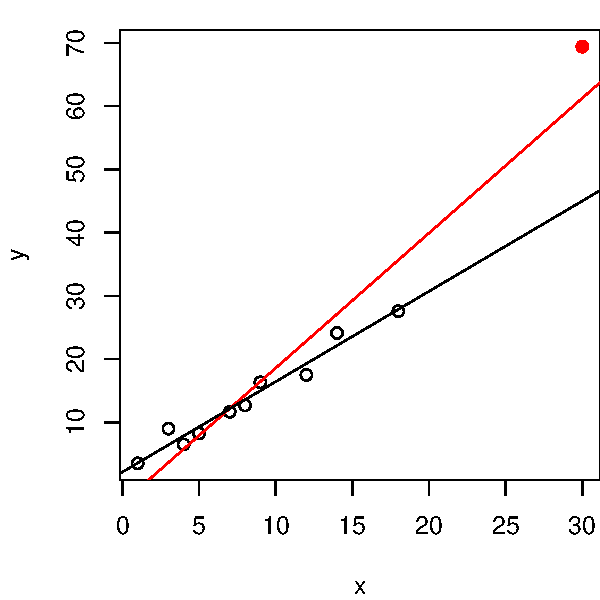
\includegraphics[width=1\linewidth]{figure/lev-1} 

\end{knitrout}
\pause
\column{0.5\linewidth}
\begin{knitrout}
\definecolor{shadecolor}{rgb}{0.969, 0.969, 0.969}\color{fgcolor}
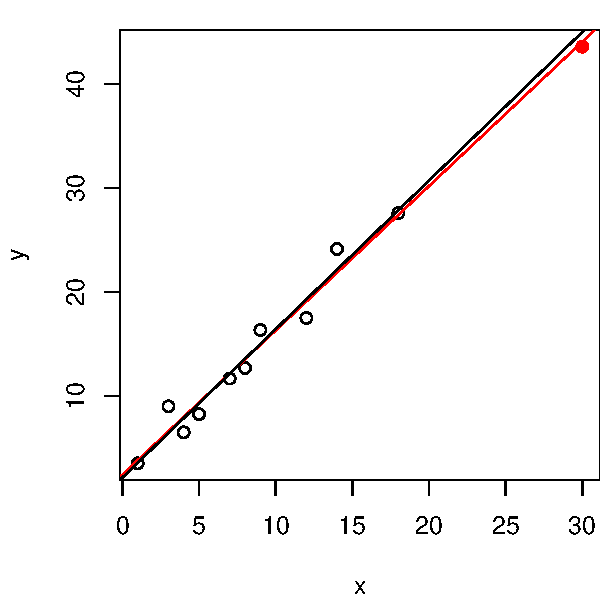
\includegraphics[width=1\linewidth]{figure/levp-1} 

\end{knitrout}
\pause
\end{columns}
\vfill
Sim, se a \emph{distância} for baixa.
\end{frame}
%============================================================================%

%===============================================================================%
\begin{frame}{Pontos Influentes}

É possível ter um ponto com \emph{distância} alta, e influência baixa? \pause
\vfill
\begin{columns}[c]

\column{0.5\linewidth}
\begin{knitrout}
\definecolor{shadecolor}{rgb}{0.969, 0.969, 0.969}\color{fgcolor}
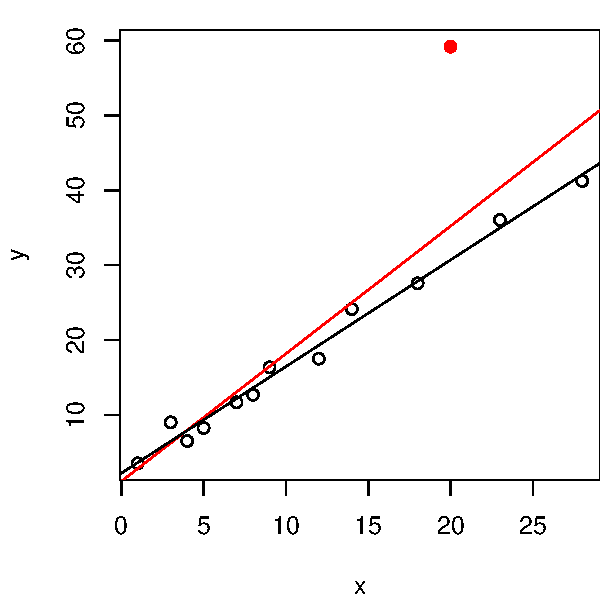
\includegraphics[width=1\linewidth]{figure/di1-1} 

\end{knitrout}
\pause
\column{0.5\linewidth}
\begin{knitrout}
\definecolor{shadecolor}{rgb}{0.969, 0.969, 0.969}\color{fgcolor}
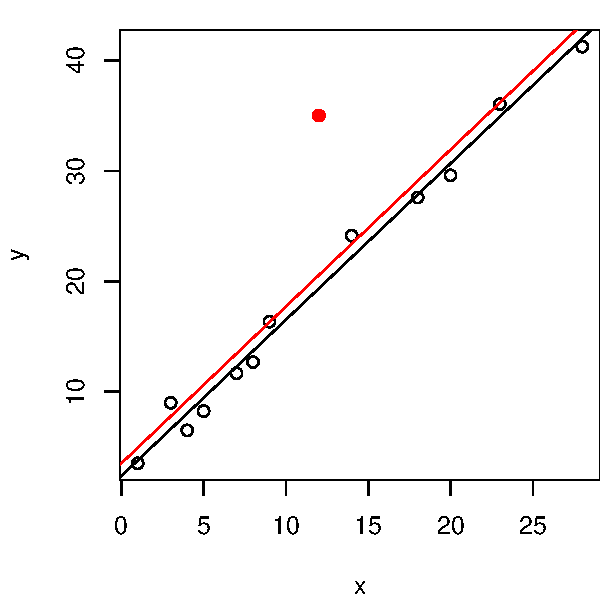
\includegraphics[width=1\linewidth]{figure/d12-1} 

\end{knitrout}
\pause
\end{columns}
\vfill
Sim, se o \emph{leverage} for baixo.

\end{frame}
%============================================================================%

%===============================================================================%
\begin{frame}{Pontos Influentes}
\small

Como identificar pontos influentes? \pause
\vfill
\textbf{DFFITS}: Diferença normalizada entre o valor de $\hat Y_i$ no modelo completo, e o valor da mesma estimativa no modelo onde o ponto $X_i,Y_i$ é removido, $\hat Y_{i(-i)}$. Identifica pontos com influência sobre estimativas de $Y$ isoladas. \pause
\vfill
\textbf{Distância de Cook}: Similar a DFFITS, mas ao invés de avaliar a diferença em um único ponto, avalia a soma dos quadrados das diferenças de todos os $\hat Y$. Identifica pontos com influência sobre todas as estimativas de $Y$. \pause
\vfill
\textbf{DFBETAS}: Diferença normalizada entre os valores dos $b$ no modelo completo, e o valor da mesma estimativa no modelo onde o ponto $X_i,Y_i$ é removido, $b_{i(-i)}$. Identifica pontos com influência sobre a inclinação da reta.

\end{frame}
%============================================================================%

%===============================================================================%
\begin{frame}{$\uparrow$ Leverage e $\uparrow$ Distance}

\begin{columns}[c]

\column{0.5\linewidth}
\begin{knitrout}
\definecolor{shadecolor}{rgb}{0.969, 0.969, 0.969}\color{fgcolor}
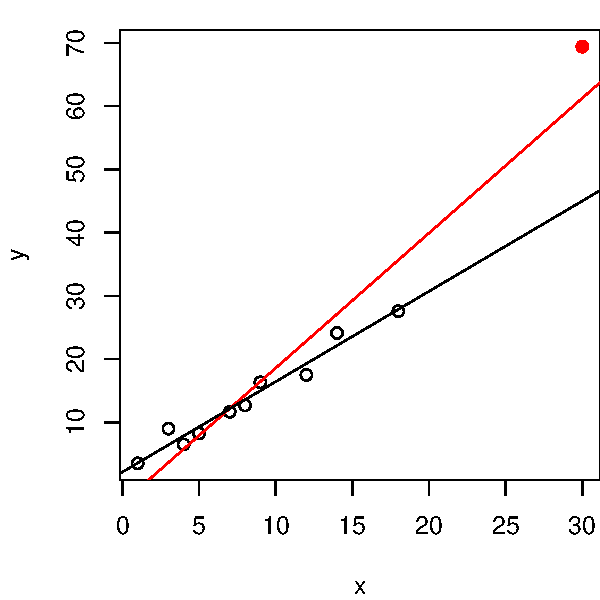
\includegraphics[width=1\linewidth]{figure/inf0-1} 

\end{knitrout}
\pause
\column{0.5\linewidth}
\begin{knitrout}\tiny
\definecolor{shadecolor}{rgb}{0.969, 0.969, 0.969}\color{fgcolor}\begin{kframe}
\begin{alltt}
\hlstd{res} \hlkwb{<-} \hlkwd{residuals}\hlstd{(m)}
\end{alltt}
\end{kframe}
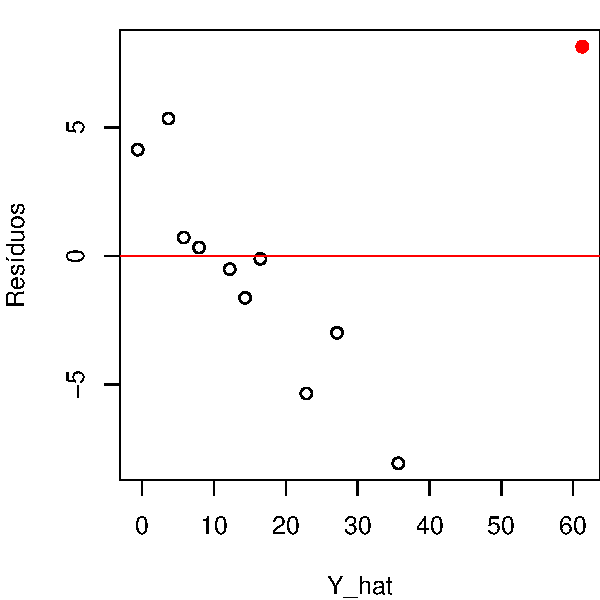
\includegraphics[width=1\linewidth]{figure/inf00-1} 

\end{knitrout}

\end{columns}
\end{frame}
%============================================================================%


%===============================================================================%
\begin{frame}{$\uparrow$ Leverage e $\uparrow$ Distance}

\begin{columns}[c]

\column{0.5\linewidth}
\begin{knitrout}
\definecolor{shadecolor}{rgb}{0.969, 0.969, 0.969}\color{fgcolor}
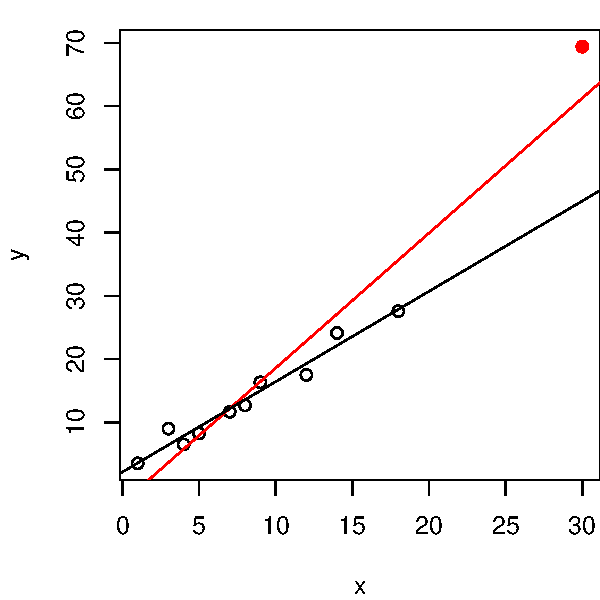
\includegraphics[width=1\linewidth]{figure/inf000-1} 

\end{knitrout}

\column{0.5\linewidth}
\begin{knitrout}\tiny
\definecolor{shadecolor}{rgb}{0.969, 0.969, 0.969}\color{fgcolor}\begin{kframe}
\begin{alltt}
\hlstd{res} \hlkwb{<-} \hlkwd{rstandard}\hlstd{(m)}
\end{alltt}
\end{kframe}
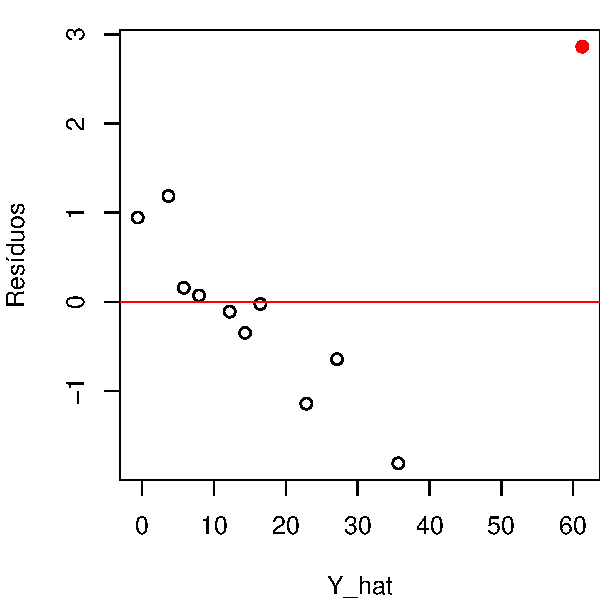
\includegraphics[width=1\linewidth]{figure/inf0000-1} 

\end{knitrout}

\end{columns}
\end{frame}
%============================================================================%

%===============================================================================%
\begin{frame}{$\uparrow$ Leverage e $\uparrow$ Distance}

\begin{columns}[c]

\column{0.5\linewidth}
\begin{knitrout}
\definecolor{shadecolor}{rgb}{0.969, 0.969, 0.969}\color{fgcolor}
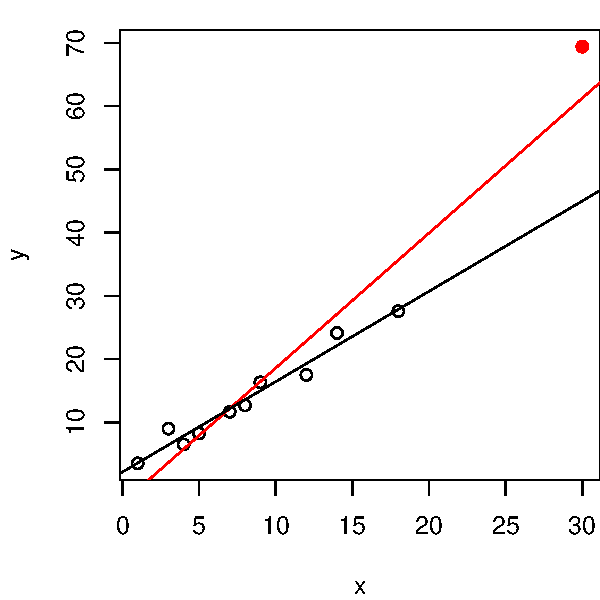
\includegraphics[width=1\linewidth]{figure/inf0-0-1} 

\end{knitrout}

\column{0.5\linewidth}
\begin{knitrout}\tiny
\definecolor{shadecolor}{rgb}{0.969, 0.969, 0.969}\color{fgcolor}\begin{kframe}
\begin{alltt}
\hlstd{res} \hlkwb{<-} \hlkwd{rstudent}\hlstd{(m)}
\end{alltt}
\end{kframe}
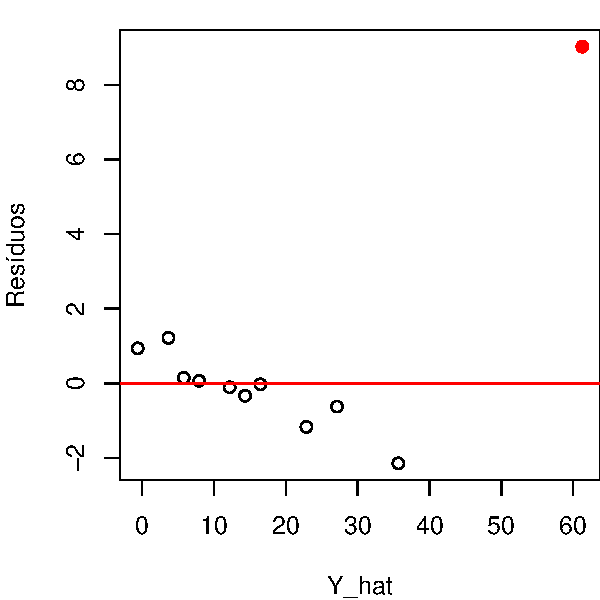
\includegraphics[width=1\linewidth]{figure/inf00-0-1} 

\end{knitrout}

\end{columns}
\end{frame}
%============================================================================%

%===============================================================================%
\begin{frame}{$\uparrow$ Leverage e $\uparrow$ Distance}

\begin{columns}[c]

\column{0.5\linewidth}
\begin{knitrout}
\definecolor{shadecolor}{rgb}{0.969, 0.969, 0.969}\color{fgcolor}
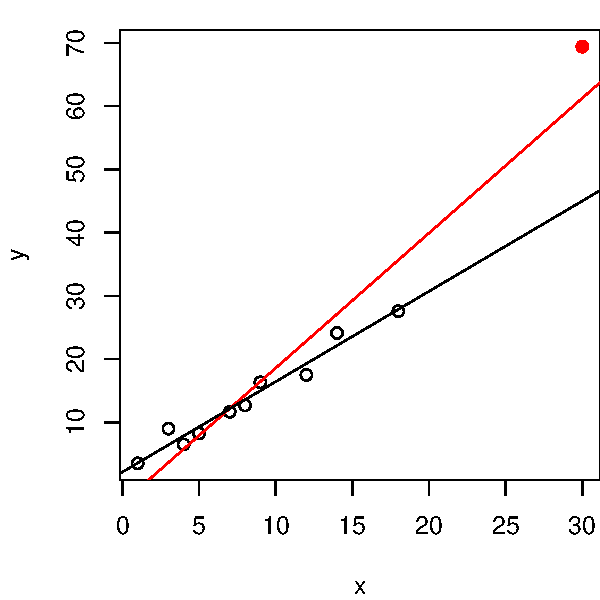
\includegraphics[width=1\linewidth]{figure/inf-1} 

\end{knitrout}

\column{0.5\linewidth}
\begin{knitrout}\tiny
\definecolor{shadecolor}{rgb}{0.969, 0.969, 0.969}\color{fgcolor}\begin{kframe}
\begin{alltt}
\hlstd{fits} \hlkwb{<-} \hlkwd{dffits}\hlstd{(m)}
\end{alltt}
\end{kframe}
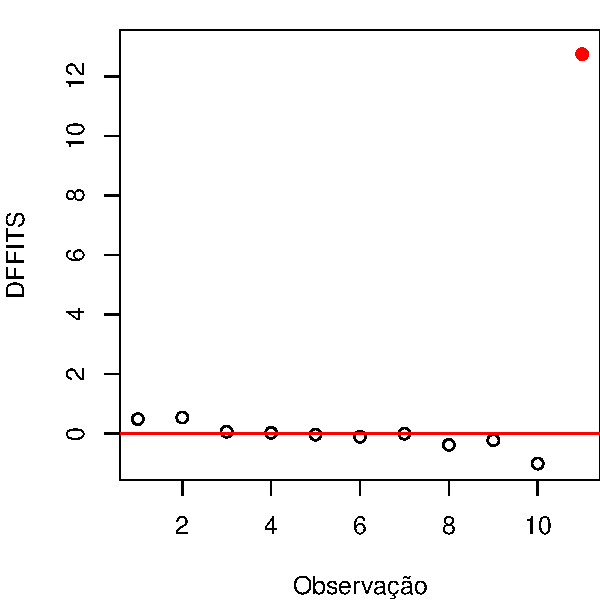
\includegraphics[width=1\linewidth]{figure/inf2-1} 

\end{knitrout}

\end{columns}
\end{frame}
%============================================================================%



%===============================================================================%
\begin{frame}{$\uparrow$ Leverage e $\uparrow$ Distance}

\begin{columns}[c]

\column{0.5\linewidth}
\begin{knitrout}
\definecolor{shadecolor}{rgb}{0.969, 0.969, 0.969}\color{fgcolor}
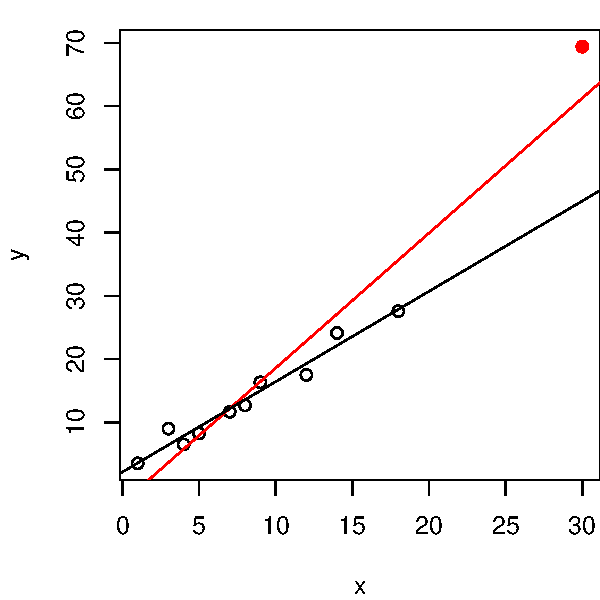
\includegraphics[width=1\linewidth]{figure/inf3-1} 

\end{knitrout}

\column{0.5\linewidth}
\begin{knitrout}\tiny
\definecolor{shadecolor}{rgb}{0.969, 0.969, 0.969}\color{fgcolor}\begin{kframe}
\begin{alltt}
\hlstd{fits} \hlkwb{<-} \hlkwd{cooks.distance}\hlstd{(m)}
\end{alltt}
\end{kframe}
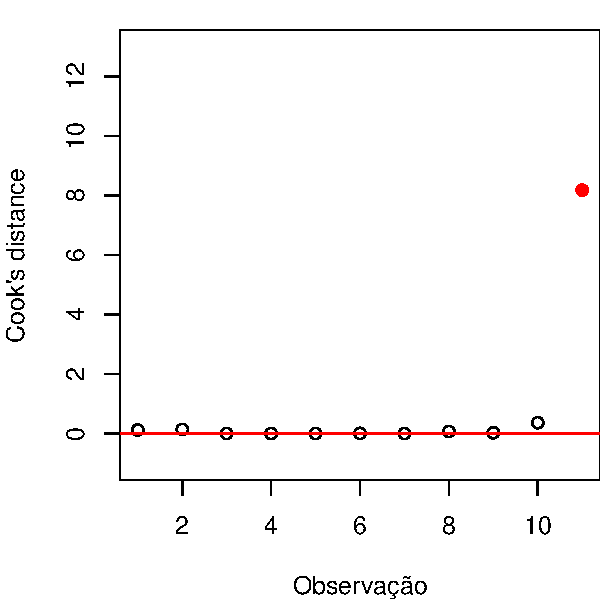
\includegraphics[width=1\linewidth]{figure/inf4-1} 

\end{knitrout}

\end{columns}
\end{frame}
%============================================================================%

%===============================================================================%
\begin{frame}{$\uparrow$ Leverage e $\uparrow$ Distance}

\begin{columns}[c]

\column{0.5\linewidth}
\begin{knitrout}
\definecolor{shadecolor}{rgb}{0.969, 0.969, 0.969}\color{fgcolor}
\includegraphics[width=1\linewidth]{figure/inf5-1} 

\end{knitrout}

\column{0.5\linewidth}
\begin{knitrout}\tiny
\definecolor{shadecolor}{rgb}{0.969, 0.969, 0.969}\color{fgcolor}\begin{kframe}
\begin{alltt}
\hlstd{fits} \hlkwb{<-} \hlkwd{dfbeta}\hlstd{(m)}
\end{alltt}
\end{kframe}
\includegraphics[width=1\linewidth]{figure/inf6-1} 

\end{knitrout}
\end{columns}
\end{frame}
%============================================================================%

%===============================================================================%
\begin{frame}{$\uparrow$ Leverage e $\uparrow$ Distance}

\begin{columns}[c]

\column{0.5\linewidth}
\begin{knitrout}
\definecolor{shadecolor}{rgb}{0.969, 0.969, 0.969}\color{fgcolor}
\includegraphics[width=1\linewidth]{figure/inf7-1} 

\end{knitrout}

\column{0.5\linewidth}
\begin{knitrout}\tiny
\definecolor{shadecolor}{rgb}{0.969, 0.969, 0.969}\color{fgcolor}\begin{kframe}
\begin{alltt}
\hlstd{fits} \hlkwb{<-} \hlkwd{dfbeta}\hlstd{(m)}
\end{alltt}
\end{kframe}
\includegraphics[width=1\linewidth]{figure/inf8-1} 

\end{knitrout}

\end{columns}
\end{frame}
%============================================================================%

%===============================================================================%
\begin{frame}{$\uparrow$ Leverage e $\downarrow$ Distance}

\begin{columns}[c]

\column{0.5\linewidth}
\begin{knitrout}
\definecolor{shadecolor}{rgb}{0.969, 0.969, 0.969}\color{fgcolor}
\includegraphics[width=1\linewidth]{figure/inf99-1} 

\end{knitrout}
\pause
\column{0.5\linewidth}
\begin{knitrout}\tiny
\definecolor{shadecolor}{rgb}{0.969, 0.969, 0.969}\color{fgcolor}\begin{kframe}
\begin{alltt}
\hlstd{res} \hlkwb{<-} \hlkwd{residuals}\hlstd{(m)}
\end{alltt}
\end{kframe}
\includegraphics[width=1\linewidth]{figure/inf109-1} 

\end{knitrout}

\end{columns}
\end{frame}
%============================================================================%

%===============================================================================%
\begin{frame}{$\uparrow$ Leverage e $\downarrow$ Distance}

\begin{columns}[c]

\column{0.5\linewidth}
\begin{knitrout}
\definecolor{shadecolor}{rgb}{0.969, 0.969, 0.969}\color{fgcolor}
\includegraphics[width=1\linewidth]{figure/inf90-1} 

\end{knitrout}

\column{0.5\linewidth}
\begin{knitrout}\tiny
\definecolor{shadecolor}{rgb}{0.969, 0.969, 0.969}\color{fgcolor}\begin{kframe}
\begin{alltt}
\hlstd{res} \hlkwb{<-} \hlkwd{rstandard}\hlstd{(m)}
\end{alltt}
\end{kframe}
\includegraphics[width=1\linewidth]{figure/inf100-1} 

\end{knitrout}

\end{columns}
\end{frame}
%============================================================================%

%===============================================================================%
\begin{frame}{$\uparrow$ Leverage e $\downarrow$ Distance}

\begin{columns}[c]

\column{0.5\linewidth}
\begin{knitrout}
\definecolor{shadecolor}{rgb}{0.969, 0.969, 0.969}\color{fgcolor}
\includegraphics[width=1\linewidth]{figure/inf91-1} 

\end{knitrout}

\column{0.5\linewidth}
\begin{knitrout}\tiny
\definecolor{shadecolor}{rgb}{0.969, 0.969, 0.969}\color{fgcolor}\begin{kframe}
\begin{alltt}
\hlstd{res} \hlkwb{<-} \hlkwd{rstudent}\hlstd{(m)}
\end{alltt}
\end{kframe}
\includegraphics[width=1\linewidth]{figure/inf101-1} 

\end{knitrout}

\end{columns}
\end{frame}
%============================================================================%

%===============================================================================%
\begin{frame}{$\uparrow$ Leverage e $\downarrow$ Distance}

\begin{columns}[c]

\column{0.5\linewidth}
\begin{knitrout}
\definecolor{shadecolor}{rgb}{0.969, 0.969, 0.969}\color{fgcolor}
\includegraphics[width=1\linewidth]{figure/inf93-1} 

\end{knitrout}

\column{0.5\linewidth}
\begin{knitrout}\tiny
\definecolor{shadecolor}{rgb}{0.969, 0.969, 0.969}\color{fgcolor}\begin{kframe}
\begin{alltt}
\hlstd{fits} \hlkwb{<-} \hlkwd{dffits}\hlstd{(m)}
\end{alltt}
\end{kframe}
\includegraphics[width=1\linewidth]{figure/inf10-1} 

\end{knitrout}

\end{columns}
\end{frame}
%============================================================================%

%===============================================================================%
\begin{frame}{$\uparrow$ Leverage e $\downarrow$ Distance}

\begin{columns}[c]

\column{0.5\linewidth}
\begin{knitrout}
\definecolor{shadecolor}{rgb}{0.969, 0.969, 0.969}\color{fgcolor}
\includegraphics[width=1\linewidth]{figure/inf11-1} 

\end{knitrout}

\column{0.5\linewidth}
\begin{knitrout}\tiny
\definecolor{shadecolor}{rgb}{0.969, 0.969, 0.969}\color{fgcolor}\begin{kframe}
\begin{alltt}
\hlstd{fits} \hlkwb{<-} \hlkwd{cooks.distance}\hlstd{(m)}
\end{alltt}
\end{kframe}
\includegraphics[width=1\linewidth]{figure/inf12-1} 

\end{knitrout}

\end{columns}
\end{frame}
%============================================================================%

%===============================================================================%
\begin{frame}{$\uparrow$ Leverage e $\downarrow$ Distance}

\begin{columns}[c]

\column{0.5\linewidth}
\begin{knitrout}
\definecolor{shadecolor}{rgb}{0.969, 0.969, 0.969}\color{fgcolor}
\includegraphics[width=1\linewidth]{figure/inf13-1} 

\end{knitrout}

\column{0.5\linewidth}
\begin{knitrout}\tiny
\definecolor{shadecolor}{rgb}{0.969, 0.969, 0.969}\color{fgcolor}\begin{kframe}
\begin{alltt}
\hlstd{fits} \hlkwb{<-} \hlkwd{dfbeta}\hlstd{(m)}
\end{alltt}
\end{kframe}
\includegraphics[width=1\linewidth]{figure/inf14-1} 

\end{knitrout}

\end{columns}
\end{frame}
%============================================================================%

%===============================================================================%
\begin{frame}{$\uparrow$ Leverage e $\downarrow$ Distance}

\begin{columns}[c]

\column{0.5\linewidth}
\begin{knitrout}
\definecolor{shadecolor}{rgb}{0.969, 0.969, 0.969}\color{fgcolor}
\includegraphics[width=1\linewidth]{figure/inf15-1} 

\end{knitrout}

\column{0.5\linewidth}
\begin{knitrout}\tiny
\definecolor{shadecolor}{rgb}{0.969, 0.969, 0.969}\color{fgcolor}\begin{kframe}
\begin{alltt}
\hlstd{fits} \hlkwb{<-} \hlkwd{dfbeta}\hlstd{(m)}
\end{alltt}
\end{kframe}
\includegraphics[width=1\linewidth]{figure/inf16-1} 

\end{knitrout}

\end{columns}
\end{frame}
%============================================================================%



%===============================================================================%
\begin{frame}{$\downarrow$ Leverage e $\uparrow$ Distance}

\begin{columns}[c]

\column{0.5\linewidth}
\begin{knitrout}
\definecolor{shadecolor}{rgb}{0.969, 0.969, 0.969}\color{fgcolor}
\includegraphics[width=1\linewidth]{figure/inf17-1} 

\end{knitrout}
\pause
\column{0.5\linewidth}
\begin{knitrout}\tiny
\definecolor{shadecolor}{rgb}{0.969, 0.969, 0.969}\color{fgcolor}\begin{kframe}
\begin{alltt}
\hlstd{res} \hlkwb{<-} \hlkwd{residuals}\hlstd{(m)}
\end{alltt}
\end{kframe}
\includegraphics[width=1\linewidth]{figure/inf200-1} 

\end{knitrout}

\end{columns}
\end{frame}
%============================================================================%

%===============================================================================%
\begin{frame}{$\uparrow$ Leverage e $\downarrow$ Distance}

\begin{columns}[c]

\column{0.5\linewidth}
\begin{knitrout}
\definecolor{shadecolor}{rgb}{0.969, 0.969, 0.969}\color{fgcolor}
\includegraphics[width=1\linewidth]{figure/inf201-1} 

\end{knitrout}

\column{0.5\linewidth}
\begin{knitrout}\tiny
\definecolor{shadecolor}{rgb}{0.969, 0.969, 0.969}\color{fgcolor}\begin{kframe}
\begin{alltt}
\hlstd{res} \hlkwb{<-} \hlkwd{rstandard}\hlstd{(m)}
\end{alltt}
\end{kframe}
\includegraphics[width=1\linewidth]{figure/inf202-1} 

\end{knitrout}

\end{columns}
\end{frame}
%============================================================================%

%===============================================================================%
\begin{frame}{$\uparrow$ Leverage e $\downarrow$ Distance}

\begin{columns}[c]

\column{0.5\linewidth}
\begin{knitrout}
\definecolor{shadecolor}{rgb}{0.969, 0.969, 0.969}\color{fgcolor}
\includegraphics[width=1\linewidth]{figure/inf203-1} 

\end{knitrout}

\column{0.5\linewidth}
\begin{knitrout}\tiny
\definecolor{shadecolor}{rgb}{0.969, 0.969, 0.969}\color{fgcolor}\begin{kframe}
\begin{alltt}
\hlstd{res} \hlkwb{<-} \hlkwd{rstudent}\hlstd{(m)}
\end{alltt}
\end{kframe}
\includegraphics[width=1\linewidth]{figure/inf204-1} 

\end{knitrout}

\end{columns}
\end{frame}
%============================================================================%

%===============================================================================%
\begin{frame}{$\uparrow$ Leverage e $\downarrow$ Distance}

\begin{columns}[c]

\column{0.5\linewidth}
\begin{knitrout}
\definecolor{shadecolor}{rgb}{0.969, 0.969, 0.969}\color{fgcolor}
\includegraphics[width=1\linewidth]{figure/inf9-1} 

\end{knitrout}

\column{0.5\linewidth}
\begin{knitrout}\tiny
\definecolor{shadecolor}{rgb}{0.969, 0.969, 0.969}\color{fgcolor}\begin{kframe}
\begin{alltt}
\hlstd{fits} \hlkwb{<-} \hlkwd{dffits}\hlstd{(m)}
\end{alltt}
\end{kframe}
\includegraphics[width=1\linewidth]{figure/inf103-1} 

\end{knitrout}

\end{columns}
\end{frame}
%============================================================================%

%===============================================================================%
\begin{frame}{$\downarrow$ Leverage e $\uparrow$ Distance}

\begin{columns}[c]

\column{0.5\linewidth}
\begin{knitrout}
\definecolor{shadecolor}{rgb}{0.969, 0.969, 0.969}\color{fgcolor}
\includegraphics[width=1\linewidth]{figure/inf19-1} 

\end{knitrout}

\column{0.5\linewidth}
\begin{knitrout}\tiny
\definecolor{shadecolor}{rgb}{0.969, 0.969, 0.969}\color{fgcolor}\begin{kframe}
\begin{alltt}
\hlstd{fits} \hlkwb{<-} \hlkwd{cooks.distance}\hlstd{(m)}
\end{alltt}
\end{kframe}
\includegraphics[width=1\linewidth]{figure/inf20-1} 

\end{knitrout}

\end{columns}
\end{frame}
%============================================================================%

%===============================================================================%
\begin{frame}{$\downarrow$ Leverage e $\uparrow$ Distance}

\begin{columns}[c]

\column{0.5\linewidth}
\begin{knitrout}
\definecolor{shadecolor}{rgb}{0.969, 0.969, 0.969}\color{fgcolor}
\includegraphics[width=1\linewidth]{figure/inf21-1} 

\end{knitrout}

\column{0.5\linewidth}
\begin{knitrout}\tiny
\definecolor{shadecolor}{rgb}{0.969, 0.969, 0.969}\color{fgcolor}\begin{kframe}
\begin{alltt}
\hlstd{fits} \hlkwb{<-} \hlkwd{dfbeta}\hlstd{(m)}
\end{alltt}
\end{kframe}
\includegraphics[width=1\linewidth]{figure/inf22-1} 

\end{knitrout}

\end{columns}
\end{frame}
%============================================================================%

%===============================================================================%
\begin{frame}{$\downarrow$ Leverage e $\uparrow$ Distance}

\begin{columns}[c]

\column{0.5\linewidth}
\begin{knitrout}
\definecolor{shadecolor}{rgb}{0.969, 0.969, 0.969}\color{fgcolor}
\includegraphics[width=1\linewidth]{figure/inf23-1} 

\end{knitrout}

\column{0.5\linewidth}
\begin{knitrout}\tiny
\definecolor{shadecolor}{rgb}{0.969, 0.969, 0.969}\color{fgcolor}\begin{kframe}
\begin{alltt}
\hlstd{fits} \hlkwb{<-} \hlkwd{dfbeta}\hlstd{(m)}
\end{alltt}
\end{kframe}
\includegraphics[width=1\linewidth]{figure/inf24-1} 

\end{knitrout}

\end{columns}
\end{frame}
%============================================================================%


%===============================================================================%
\begin{frame}{$\downarrow$ Leverage e $\uparrow$ Distance}

Visualização + diagnóstico!

\begin{columns}[c]

\column{0.5\linewidth}
\begin{knitrout}
\definecolor{shadecolor}{rgb}{0.969, 0.969, 0.969}\color{fgcolor}
\includegraphics[width=1\linewidth]{figure/inf25-1} 

\end{knitrout}

\column{0.55\linewidth}
\begin{knitrout}\tiny
\definecolor{shadecolor}{rgb}{0.969, 0.969, 0.969}\color{fgcolor}
\includegraphics[width=1\linewidth]{figure/inf26-1} 

\end{knitrout}

\end{columns}
\end{frame}
%============================================================================%


%===============================================================================%
\begin{frame}{\emph{Testes Estatísticos para Pressuposições}}

Os modelos lineares gerais são robustos, e podem tolerar pequenos desvios. Mas se voce realmente quer testar...\pause
\vfill
\begin{itemize}
\item \textbf{Normalidade:} Kolmogorov-Smirnov, Shapiro-Wilk, Lilliefors
\vfill
\item \textbf{Heteroscedasticidade:} Breusch-Pagan, White
\vfill
\item \textbf{Independência:} Durbin-Watson, Função de Autocorrelação
\vfill
\end{itemize}
\end{frame}
%===============================================================================%

\section{Remediação}


%===============================================================================%
\begin{frame}{Remediação}

Após a análise diagnóstica, descobrimos que nosso modelo viola uma ou mais pressuposições. O que fazer? \pause
\vfill
\begin{itemize}
  \item Transformação de variáveis \pause
  \vfill
  \item Métodos Robustos e/ou Não-Paramétricos (outra aula)\pause
  \vfill
  \item Outros modelos que não Modelos Lineares Gerais (outra aula)\pause
  \vfill
  \item Métodos de aleatorização e reamostragem 
\end{itemize}
  
\end{frame}
%===============================================================================%


%===============================================================================%
\begin{frame}{Transformação de Variáveis}

A alternativa mais simples para violações dos pressupostos é a transformação de variáveis \pause
\vfill
Mas\ldots se transformarmos as variáveis originais, não vamos alterar a relação entre elas? \pause
\vfill
As transformações devem ser \textbf{monotônicas} (preservam a ordem relativa dos dados): Se $ X_i > X_j$, então $f(X_i) > f(X_j)$, e vice versa. \pause
\vfill
Se usarmos funções monotônicas, podemos alterar a distância relativa entre os pontos, e assim a variância e a forma da distribuição 
  
\end{frame}
%===============================================================================%


%===============================================================================%
\begin{frame}{Funções de potência}

A família de funções de potência oferece flexibilidade, dentro de uma mesma especificação: \pause
\vfill
$Y' = cY^\lambda$ inclui: \pause
\vfill
\begin{itemize}
\item $Y^{-\lambda} = \dfrac{1}{Y^\lambda}$ \pause, se $\lambda = 1$, $Y' = Y^{-1} = 1/Y$ \pause
\vfill
\item $Y^{\frac{1}{\lambda}} = \sqrt[\lambda]{Y}$ \pause
\vfill
\item $Y^\lambda$ \pause
\end{itemize}
\vfill
$c$ é apenas uma constante de escala
  
\end{frame}
%===============================================================================%


%===============================================================================%
\begin{frame}{Funções de potência}

As relações de potência podem também ser expressas na forma abaixo, conhecida como transformação de Box-Cox \pause
\vfill
$ Y' = \frac{Y^\lambda - 1}{\lambda}$, para $\lambda \neq 0$  \pause
\vfill
$Y' = log(Y)$, para $\lambda = 0$ \pause
\vfill
A expressão acima é válida pois $\lim_{\lambda \to 0} \frac{Y^\lambda - 1}{\lambda} = \log _e (X)$ \pause
\vfill
Normalmente se prefere $\log _{10}$ para facilitar a interpretação, pois um aumento de 1 em $\log _{10}(Y)$ é o mesmo que multiplicar $Y$ por 10
  
\end{frame}
%===============================================================================%

%===============================================================================%
\begin{frame}{Regra da Convexidade de Tukey}


\centering

\includegraphics[width=0.8\linewidth]{TukeyBulge.png}


\end{frame}
%===============================================================================%

%===============================================================================%
\begin{frame}{Regra da Convexidade de Tukey}

\begin{columns}[c]

\column{0.5\linewidth}
\centering
\includegraphics[width=1.3\linewidth]{TukeyBulge.png}

\column{0.8\linewidth}
\centering
\begin{knitrout}
\definecolor{shadecolor}{rgb}{0.969, 0.969, 0.969}\color{fgcolor}
\includegraphics[width=0.7\linewidth]{figure/rem1-1} 

\end{knitrout}

\end{columns}

\end{frame}
%===============================================================================%


%===============================================================================%
\begin{frame}{Regra da Convexidade de Tukey}

\begin{columns}[c]

\column{0.5\linewidth}
\centering
\includegraphics[width=1.3\linewidth]{TukeyBulge.png}

\column{0.8\linewidth}
\centering
\begin{knitrout}\scriptsize
\definecolor{shadecolor}{rgb}{0.969, 0.969, 0.969}\color{fgcolor}\begin{kframe}
\begin{alltt}
\hlkwd{plot}\hlstd{(x,}\hlkwd{sqrt}\hlstd{(y))}
\end{alltt}
\end{kframe}
\includegraphics[width=0.7\linewidth]{figure/rem2-1} 

\end{knitrout}

\end{columns}

\end{frame}
%===============================================================================%


%===============================================================================%
\begin{frame}{Regra da Convexidade de Tukey}

\begin{columns}[c]

\column{0.5\linewidth}
\centering
\includegraphics[width=1.3\linewidth]{TukeyBulge.png}

\column{0.8\linewidth}
\centering
\begin{knitrout}\scriptsize
\definecolor{shadecolor}{rgb}{0.969, 0.969, 0.969}\color{fgcolor}\begin{kframe}
\begin{alltt}
\hlkwd{plot}\hlstd{(x,}\hlkwd{log10}\hlstd{(y))}
\end{alltt}
\end{kframe}
\includegraphics[width=0.7\linewidth]{figure/rem3-1} 

\end{knitrout}

\end{columns}

\end{frame}
%===============================================================================%

%===============================================================================%
\begin{frame}{Regra da Convexidade de Tukey}

\begin{columns}[c]

\column{0.5\linewidth}
\centering
\includegraphics[width=1.3\linewidth]{TukeyBulge.png}

\column{0.8\linewidth}
\centering
\begin{knitrout}\scriptsize
\definecolor{shadecolor}{rgb}{0.969, 0.969, 0.969}\color{fgcolor}\begin{kframe}
\begin{alltt}
\hlkwd{plot}\hlstd{(x}\hlopt{^}\hlnum{2}\hlstd{,y)}
\end{alltt}
\end{kframe}
\includegraphics[width=0.7\linewidth]{figure/rem4-1} 

\end{knitrout}

\end{columns}

\end{frame}
%===============================================================================%

%===============================================================================%
\begin{frame}{Regra da Convexidade de Tukey}

\begin{columns}[c]

\column{0.5\linewidth}
\centering
\includegraphics[width=1.3\linewidth]{TukeyBulge.png}

\column{0.8\linewidth}
\centering
\begin{knitrout}\scriptsize
\definecolor{shadecolor}{rgb}{0.969, 0.969, 0.969}\color{fgcolor}\begin{kframe}
\begin{alltt}
\hlkwd{plot}\hlstd{(x}\hlopt{^}\hlnum{3}\hlstd{,y)}
\end{alltt}
\end{kframe}
\includegraphics[width=0.7\linewidth]{figure/rem5-1} 

\end{knitrout}

\end{columns}

\end{frame}
%===============================================================================%

%===============================================================================%
\begin{frame}{Regra da Convexidade de Tukey}

\begin{columns}[c]

\column{0.5\linewidth}
\centering
\includegraphics[width=1.3\linewidth]{TukeyBulge.png}

\column{0.8\linewidth}
\centering
\begin{knitrout}
\definecolor{shadecolor}{rgb}{0.969, 0.969, 0.969}\color{fgcolor}
\includegraphics[width=0.7\linewidth]{figure/rem6-1} 

\end{knitrout}

\end{columns}

\end{frame}
%===============================================================================%

%===============================================================================%
\begin{frame}{Regra da Convexidade de Tukey}

\begin{columns}[c]

\column{0.5\linewidth}
\centering
\includegraphics[width=1.3\linewidth]{TukeyBulge.png}

\column{0.8\linewidth}
\centering
\begin{knitrout}
\definecolor{shadecolor}{rgb}{0.969, 0.969, 0.969}\color{fgcolor}
\includegraphics[width=0.7\linewidth]{figure/rem7-1} 

\end{knitrout}

\end{columns}

\end{frame}
%===============================================================================%

%===============================================================================%
\begin{frame}{Regra da Convexidade de Tukey}

\begin{columns}[c]

\column{0.5\linewidth}
\centering
\includegraphics[width=1.3\linewidth]{TukeyBulge.png}

\column{0.8\linewidth}
\centering
\begin{knitrout}
\definecolor{shadecolor}{rgb}{0.969, 0.969, 0.969}\color{fgcolor}
\includegraphics[width=0.7\linewidth]{figure/rem8-1} 

\end{knitrout}

\end{columns}

\end{frame}
%===============================================================================%

%===============================================================================%
\begin{frame}{Regra da Convexidade de Tukey}

\begin{columns}[c]

\column{0.5\linewidth}
\centering
\includegraphics[width=1.3\linewidth]{TukeyBulge.png}

\column{0.8\linewidth}
\centering
\begin{knitrout}
\definecolor{shadecolor}{rgb}{0.969, 0.969, 0.969}\color{fgcolor}
\includegraphics[width=0.7\linewidth]{figure/rem9-1} 

\end{knitrout}

\end{columns}

\end{frame}
%===============================================================================%

%===============================================================================%
\begin{frame}{Regra da Convexidade de Tukey}

\begin{columns}[c]

\column{0.5\linewidth}
\centering
\includegraphics[width=1.3\linewidth]{TukeyBulge.png}

\column{0.8\linewidth}
\centering
\begin{knitrout}
\definecolor{shadecolor}{rgb}{0.969, 0.969, 0.969}\color{fgcolor}
\includegraphics[width=0.7\linewidth]{figure/rem20-1} 

\end{knitrout}

\end{columns}

\end{frame}
%===============================================================================%



%===============================================================================%
\begin{frame}[fragile]{Otimização de $\lambda$}

 Podemos utilizar métodos computacionais para encontrar o melhor valor de $\lambda$ (médodo de máxima verossimilhança, \emph(maximum likelihood)

\begin{columns}[c]

\column{0.5\linewidth}

\begin{knitrout}\tiny
\definecolor{shadecolor}{rgb}{0.969, 0.969, 0.969}\color{fgcolor}\begin{kframe}
\begin{alltt}
\hlstd{x} \hlkwb{<-} \hlkwd{c}\hlstd{(}\hlnum{1}\hlopt{:}\hlnum{30}\hlstd{)}
\hlstd{y} \hlkwb{<-} \hlnum{2} \hlopt{+} \hlstd{x}\hlopt{^}\hlnum{2.786}
\hlstd{m} \hlkwb{<-}\hlkwd{lm}\hlstd{(y}\hlopt{~}\hlstd{x)}
\hlkwd{plot}\hlstd{(x,y)}
\hlkwd{abline}\hlstd{(m)}
\end{alltt}
\end{kframe}
\end{knitrout}

\column{0.5\linewidth}

\centering
\begin{knitrout}\scriptsize
\definecolor{shadecolor}{rgb}{0.969, 0.969, 0.969}\color{fgcolor}
\includegraphics[width=0.9\linewidth]{figure/oti2-1} 

\end{knitrout}

\end{columns}

\end{frame}
%===============================================================================%


%===============================================================================%
\begin{frame}[fragile]{Otimização de $\lambda$}

 Podemos utilizar métodos computacionais para encontrar o melhor valor de $\lambda$ (médodo de máxima verossimilhança, ou \emph{maximum likelihood})

\begin{columns}[c]

\column{0.5\linewidth}

\begin{knitrout}\tiny
\definecolor{shadecolor}{rgb}{0.969, 0.969, 0.969}\color{fgcolor}\begin{kframe}
\begin{alltt}
\hlkwd{library}\hlstd{(MASS)}
\hlstd{lambda} \hlkwb{<-} \hlkwd{boxcox}\hlstd{(m)}
\end{alltt}
\end{kframe}
\end{knitrout}


\column{0.5\linewidth}
\centering
\begin{knitrout}\scriptsize
\definecolor{shadecolor}{rgb}{0.969, 0.969, 0.969}\color{fgcolor}
\includegraphics[width=0.9\linewidth]{figure/oti4-1} 

\end{knitrout}

\end{columns}

\end{frame}
%===============================================================================%
% 
% 
%===============================================================================%
\begin{frame}[fragile]{Otimização de $\lambda$}

 Podemos utilizar métodos computacionais para encontrar o melhor valor de $\lambda$ (médodo de máxima verossimilhança, \emph(maximum likelihood)

\begin{columns}[c]

\column{0.5\linewidth}

\begin{knitrout}\tiny
\definecolor{shadecolor}{rgb}{0.969, 0.969, 0.969}\color{fgcolor}\begin{kframe}
\begin{alltt}
\hlkwd{which}\hlstd{(lambda}\hlopt{$}\hlstd{y} \hlopt{==} \hlkwd{max}\hlstd{(lambda}\hlopt{$}\hlstd{y))}
\end{alltt}
\begin{verbatim}
## [1] 59
\end{verbatim}
\begin{alltt}
\hlstd{lambda}\hlopt{$}\hlstd{x[}\hlnum{59}\hlstd{]}
\end{alltt}
\begin{verbatim}
## [1] 0.3434343
\end{verbatim}
\begin{alltt}
\hlstd{newy} \hlkwb{<-} \hlstd{(y}\hlopt{^}\hlnum{0.3434343} \hlopt{-}\hlnum{1}\hlstd{)}\hlopt{/}\hlnum{0.3434343}
\hlkwd{plot}\hlstd{(x,newy)}
\end{alltt}
\end{kframe}
\end{knitrout}


\column{0.5\linewidth}
\centering

\begin{knitrout}\scriptsize
\definecolor{shadecolor}{rgb}{0.969, 0.969, 0.969}\color{fgcolor}
\includegraphics[width=0.9\linewidth]{figure/oti6-1} 

\end{knitrout}

\end{columns}

\end{frame}
%===============================================================================%


%===============================================================================%
\begin{frame}{Transformações: normalidade e variância}

 O uso de transformações não se limita à linearização de variáveis, mas também é de grande ajuda na aproximação dos dados para uma distribuição normal e variância constante
\begin{columns}[c]

\column{0.5\linewidth}

\begin{knitrout}\scriptsize
\definecolor{shadecolor}{rgb}{0.969, 0.969, 0.969}\color{fgcolor}
\includegraphics[width=0.9\linewidth]{figure/t1-1} 

\end{knitrout}


\column{0.5\linewidth}
\centering

\begin{knitrout}\scriptsize
\definecolor{shadecolor}{rgb}{0.969, 0.969, 0.969}\color{fgcolor}
\includegraphics[width=0.9\linewidth]{figure/t2-1} 

\end{knitrout}

\end{columns}

\end{frame}
%===============================================================================%



%===============================================================================%
\begin{frame}{Transformações: normalidade e variância}

 O uso de transformações não se limita à linearização de variáveis, mas também é de grande ajuda na aproximação dos dados para uma distribuição normal e variância constante
\begin{columns}[c]

\column{0.5\linewidth}

\begin{knitrout}\scriptsize
\definecolor{shadecolor}{rgb}{0.969, 0.969, 0.969}\color{fgcolor}
\includegraphics[width=0.9\linewidth]{figure/t3-1} 

\end{knitrout}


\column{0.5\linewidth}
\centering

\begin{knitrout}\scriptsize
\definecolor{shadecolor}{rgb}{0.969, 0.969, 0.969}\color{fgcolor}
\includegraphics[width=0.9\linewidth]{figure/t4-1} 

\end{knitrout}

\end{columns}

\end{frame}
%===============================================================================%

\section{Validação}


%===============================================================================%
\begin{frame}{Validação}

Já fizemos a análise exploratória, ajustamos o modelo, analisamos os resíduos, resolvemos problemas de violação das pressuposições. Nosso modelo está pronto. \pause
\vfill
E agora?\pause
\vfill
A última etapa do processo de modelagem consiste na \textbf{validação}, isto é, avaliação da ``veracidade'' do modelo \pause
\vfill
Se o modelo é explicativo, queremos ter certeza sobre nossos coeficientes \pause
\vfill
Se o modelo é preditivo, queremos ter certeza sobre as novas predições 

\end{frame}
%===============================================================================%


%===============================================================================%
\begin{frame}{Validação}

Os coeficientes do nosso modelo explicam a relação entre $X$ e $Y$, e através desta relação podemos prever novos valores de $Y$ \pause
\vfill
Mas o quanto podemos confiar em $b_0$ e $b_1$ como estimativas de $\beta _0$ e $\beta _1$, e nos valores de $\hat Y_{i(novo)}$ ? \pause
\vfill
1) Intervalos de confiança paramétricos \pause
\vfill
2) Validação independente \pause
\vfill
3) Métodos de aleatorização e reamostragem

\end{frame}
%===============================================================================%


%===============================================================================%
\begin{frame}[fragile]{Exemplo}

 Distância de frenagem pode ser predita pela velocidade do veículo?

\begin{columns}[c]

\column{0.6\linewidth}

\begin{knitrout}\tiny
\definecolor{shadecolor}{rgb}{0.969, 0.969, 0.969}\color{fgcolor}\begin{kframe}
\begin{alltt}
\hlkwd{summary}\hlstd{(m0)}
\end{alltt}
\begin{verbatim}
## 
## Call:
## lm(formula = dist ~ speed, data = cars)
## 
## Residuals:
##     Min      1Q  Median      3Q     Max 
## -8.8603 -2.9033 -0.6925  2.8086 13.1678 
## 
## Coefficients:
##             Estimate Std. Error t value Pr(>|t|)    
## (Intercept)  -5.3581     2.0600  -2.601   0.0123 *  
## speed         0.7448     0.0787   9.464 1.49e-12 ***
## ---
## Signif. codes:  0 '***' 0.001 '**' 0.01 '*' 0.05 '.' 0.1 ' ' 1
## 
## Residual standard error: 4.688 on 48 degrees of freedom
## Multiple R-squared:  0.6511,	Adjusted R-squared:  0.6438 
## F-statistic: 89.57 on 1 and 48 DF,  p-value: 1.49e-12
\end{verbatim}
\end{kframe}
\end{knitrout}

\column{0.4\linewidth}

\begin{knitrout}\scriptsize
\definecolor{shadecolor}{rgb}{0.969, 0.969, 0.969}\color{fgcolor}
\includegraphics[width=1\linewidth]{figure/v2-1} 

\end{knitrout}

\end{columns}

\end{frame}
%===============================================================================%

%===============================================================================%
\begin{frame}{Validação Cruzada com Dados Independentes}

A melhor medida da capacidade de predição do modelo é a sua performance em estimar valores não usados no ajuste \pause
\vfill
Mas ao mesmo tempo, queremos usar o máximo de observações possíveis, para ter o melhor ajuste \pause

\vfill
\textbf{Validação cruzada:} dividimos a amostra em 2 partes iguais, e usamos cada metade para validar um modelo ajustado à outra metade

\end{frame}
%===============================================================================%


%===============================================================================%
\begin{frame}[fragile]{Exemplo}

 Distância de frenagem pode ser predita pela velocidade do veículo?

\begin{columns}[c]

\column{0.6\linewidth}

\begin{knitrout}\tiny
\definecolor{shadecolor}{rgb}{0.969, 0.969, 0.969}\color{fgcolor}\begin{kframe}
\begin{alltt}
\hlkwd{dim}\hlstd{(cars)}
\end{alltt}
\begin{verbatim}
## [1] 50  2
\end{verbatim}
\begin{alltt}
\hlkwd{set.seed}\hlstd{(}\hlnum{89}\hlstd{)}
\hlstd{samp} \hlkwb{<-} \hlkwd{sample}\hlstd{(}\hlnum{1}\hlopt{:}\hlnum{50}\hlstd{,}\hlnum{25}\hlstd{,}\hlkwc{rep}\hlstd{=F)}
\hlstd{cars1} \hlkwb{<-} \hlstd{cars[samp,]}
\hlstd{cars2} \hlkwb{<-} \hlstd{cars[}\hlopt{-}\hlstd{samp,]}
\hlstd{m1} \hlkwb{<-} \hlkwd{lm}\hlstd{(dist} \hlopt{~} \hlstd{speed, cars1)}
\hlstd{m2} \hlkwb{<-} \hlkwd{lm}\hlstd{(dist} \hlopt{~} \hlstd{speed, cars2)}
\end{alltt}
\end{kframe}
\end{knitrout}

\column{0.4\linewidth}

\begin{knitrout}\scriptsize
\definecolor{shadecolor}{rgb}{0.969, 0.969, 0.969}\color{fgcolor}
\includegraphics[width=.7\linewidth]{figure/v4-1} 

\includegraphics[width=.7\linewidth]{figure/v4-2} 

\end{knitrout}

\end{columns}

\end{frame}
%===============================================================================%


%===============================================================================%
\begin{frame}[fragile]{Exemplo}

 Distância de frenagem pode ser predita pela velocidade do veículo?

\begin{columns}[c]

\column{0.6\linewidth}

\begin{knitrout}\tiny
\definecolor{shadecolor}{rgb}{0.969, 0.969, 0.969}\color{fgcolor}\begin{kframe}
\begin{alltt}
\hlkwd{summary}\hlstd{(m1)}\hlopt{$}\hlstd{coefficients}
\end{alltt}
\begin{verbatim}
##               Estimate Std. Error   t value     Pr(>|t|)
## (Intercept) -3.6299189 2.45699491 -1.477382 1.531367e-01
## speed        0.6699674 0.08863644  7.558600 1.119803e-07
\end{verbatim}
\begin{alltt}
\hlkwd{summary}\hlstd{(m2)}\hlopt{$}\hlstd{coefficients}
\end{alltt}
\begin{verbatim}
##               Estimate Std. Error   t value     Pr(>|t|)
## (Intercept) -7.9600734  3.4865900 -2.283054 3.199371e-02
## speed        0.8660454  0.1421012  6.094569 3.235797e-06
\end{verbatim}
\end{kframe}
\end{knitrout}

\column{0.4\linewidth}

\begin{knitrout}\scriptsize
\definecolor{shadecolor}{rgb}{0.969, 0.969, 0.969}\color{fgcolor}
\includegraphics[width=.7\linewidth]{figure/v6-1} 

\includegraphics[width=.7\linewidth]{figure/v6-2} 

\end{knitrout}

\end{columns}

\end{frame}
%===============================================================================%


%===============================================================================%
\begin{frame}[fragile]{Exemplo}

 Distância de frenagem pode ser predita pela velocidade do veículo?

\begin{columns}[c]

\column{0.6\linewidth}

\begin{knitrout}\tiny
\definecolor{shadecolor}{rgb}{0.969, 0.969, 0.969}\color{fgcolor}\begin{kframe}
\begin{alltt}
\hlstd{pr1} \hlkwb{<-} \hlkwd{predict}\hlstd{(m1,cars2)}
\hlstd{pr2} \hlkwb{<-}\hlkwd{predict}\hlstd{(m2,cars1)}
\hlstd{rmse1} \hlkwb{<-} \hlkwd{sqrt}\hlstd{(}\hlkwd{mean}\hlstd{((cars2}\hlopt{$}\hlstd{dist} \hlopt{-} \hlstd{pr1)}\hlopt{^}\hlnum{2}\hlstd{))}
\hlstd{rmse2} \hlkwb{<-} \hlkwd{sqrt}\hlstd{(}\hlkwd{mean}\hlstd{((cars1}\hlopt{$}\hlstd{dist} \hlopt{-} \hlstd{pr2)}\hlopt{^}\hlnum{2}\hlstd{))}
\hlstd{rmse1}
\end{alltt}
\begin{verbatim}
## [1] 5.311186
\end{verbatim}
\begin{alltt}
\hlstd{rmse2}
\end{alltt}
\begin{verbatim}
## [1] 4.313988
\end{verbatim}
\end{kframe}
\end{knitrout}

\column{0.4\linewidth}

\begin{knitrout}\scriptsize
\definecolor{shadecolor}{rgb}{0.969, 0.969, 0.969}\color{fgcolor}
\includegraphics[width=.7\linewidth]{figure/v8-1} 

\includegraphics[width=.7\linewidth]{figure/v8-2} 

\end{knitrout}

\end{columns}

\end{frame}
%===============================================================================%

%===============================================================================%
\begin{frame}{\emph{Jackknife} ou \emph{LOOCV}}

Não seria ótimo se pudéssemos usar o máximo possível de observações pra estimar o erro? \pause
\vfill
E se, ao invés de dividir meio a meio, deixássemos uma observação de fora, e repetíssemos $n$ vezes? \pause

\vfill
\textbf{\emph{Jacknife} ou \emph{Leave One Out Cross-Validation (LOOCV)}} 

\end{frame}
%===============================================================================%

%===============================================================================%
\begin{frame}[fragile]{Exemplo}

 Distância de frenagem pode ser predita pela velocidade do veículo?

\begin{columns}[c]

\column{0.6\linewidth}

\begin{knitrout}\tiny
\definecolor{shadecolor}{rgb}{0.969, 0.969, 0.969}\color{fgcolor}\begin{kframe}
\begin{alltt}
\hlstd{b0} \hlkwb{<-} \hlkwd{vector}\hlstd{()}
\hlstd{b1} \hlkwb{<-} \hlkwd{vector}\hlstd{()}
\hlstd{rq} \hlkwb{<-} \hlkwd{vector}\hlstd{()}
\hlkwa{for} \hlstd{(i} \hlkwa{in} \hlkwd{c}\hlstd{(}\hlnum{1}\hlopt{:}\hlnum{50}\hlstd{))\{}
  \hlstd{m} \hlkwb{<-} \hlkwd{lm}\hlstd{(dist} \hlopt{~} \hlstd{speed,} \hlkwc{data}\hlstd{=cars[}\hlopt{-}\hlstd{i,])}
  \hlstd{b0} \hlkwb{<-} \hlkwd{c}\hlstd{(b0,}\hlkwd{coefficients}\hlstd{(m)[}\hlnum{1}\hlstd{])}
  \hlstd{b1} \hlkwb{<-} \hlkwd{c}\hlstd{(b1,}\hlkwd{coefficients}\hlstd{(m)[}\hlnum{2}\hlstd{])}
  \hlstd{rq} \hlkwb{<-} \hlkwd{c}\hlstd{(rq,}\hlkwd{summary}\hlstd{(m)}\hlopt{$}\hlstd{r.squared)}
\hlstd{\}}
\end{alltt}
\end{kframe}
\end{knitrout}

\column{0.4\linewidth}

\begin{knitrout}\scriptsize
\definecolor{shadecolor}{rgb}{0.969, 0.969, 0.969}\color{fgcolor}
\includegraphics[width=.7\linewidth]{figure/v10-1} 

\includegraphics[width=.7\linewidth]{figure/v10-2} 

\end{knitrout}

\end{columns}

\end{frame}
%===============================================================================%


%===============================================================================%
\begin{frame}[fragile]{Exemplo}

 Distância de frenagem pode ser predita pela velocidade do veículo?

\begin{columns}[c]

\column{0.6\linewidth}

\begin{knitrout}\tiny
\definecolor{shadecolor}{rgb}{0.969, 0.969, 0.969}\color{fgcolor}\begin{kframe}
\begin{alltt}
\hlstd{pred} \hlkwb{<-} \hlstd{b0} \hlopt{+} \hlstd{cars}\hlopt{$}\hlstd{speed} \hlopt{*} \hlstd{b1}
\hlstd{erro} \hlkwb{<-} \hlstd{cars}\hlopt{$}\hlstd{dist}\hlopt{-}\hlstd{pred}
\hlstd{rmse} \hlkwb{<-} \hlkwd{sqrt}\hlstd{(}\hlkwd{mean}\hlstd{(erro}\hlopt{^}\hlnum{2}\hlstd{))}
\hlstd{rmse}
\end{alltt}
\begin{verbatim}
## [1] 4.784539
\end{verbatim}
\end{kframe}
\end{knitrout}

\column{0.4\linewidth}

\begin{knitrout}\scriptsize
\definecolor{shadecolor}{rgb}{0.969, 0.969, 0.969}\color{fgcolor}
\includegraphics[width=.7\linewidth]{figure/v12-1} 

\includegraphics[width=.7\linewidth]{figure/v12-2} 

\end{knitrout}

\end{columns}

\end{frame}
%===============================================================================%


%===============================================================================%
\begin{frame}{\emph{Jackknife} ou \emph{LOOCV}}

Esse método pode também ser usado para criar intervalos de confiança para $\beta _0$, $\beta _1$, etc. \pause
\vfill
Conduza a aleatorização, e reporte os percentis $\alpha/2$ e $1-\alpha/2$ \pause

\vfill

\textbf{Problema:} poucas observações

\end{frame}
%===============================================================================%


%===============================================================================%
\begin{frame}{\emph{Bootstrap}}

\textbf{Bootstrap}

Generalização dos métodos de reamostragem \pause
\vfill
Selecione $n$ novas amostras, com reposição, e recalcule o modelo. Repita \textbf{muitas} vezes. \pause

\vfill

Observações mais frequentes vão ser reamostradas mais vezes \pause

\vfill

O resultado final aproxima a distribuição original de $\varepsilon$ e $Y$ (seja ela qual for)

\end{frame}
%===============================================================================%


%===============================================================================%
\begin{frame}[fragile]{Exemplo}

 Distância de frenagem pode ser predita pela velocidade do veículo?

\begin{columns}[c]

\column{0.6\linewidth}

\begin{knitrout}\tiny
\definecolor{shadecolor}{rgb}{0.969, 0.969, 0.969}\color{fgcolor}\begin{kframe}
\begin{alltt}
\hlstd{b0} \hlkwb{<-} \hlkwd{vector}\hlstd{()}
\hlstd{b1} \hlkwb{<-} \hlkwd{vector}\hlstd{()}
\hlstd{rq} \hlkwb{<-} \hlkwd{vector}\hlstd{()}
\hlkwa{for} \hlstd{(i} \hlkwa{in} \hlkwd{c}\hlstd{(}\hlnum{1}\hlopt{:}\hlnum{1000}\hlstd{))\{}
  \hlstd{sub} \hlkwb{<-} \hlkwd{sample}\hlstd{(}\hlnum{1}\hlopt{:}\hlnum{50}\hlstd{,}\hlnum{50}\hlstd{,}\hlkwc{replace}\hlstd{=T)}
  \hlstd{m} \hlkwb{<-} \hlkwd{lm}\hlstd{(dist} \hlopt{~} \hlstd{speed,} \hlkwc{data}\hlstd{=cars[sub,])}
  \hlstd{b0} \hlkwb{<-} \hlkwd{c}\hlstd{(b0,}\hlkwd{coefficients}\hlstd{(m)[}\hlnum{1}\hlstd{])}
  \hlstd{b1} \hlkwb{<-} \hlkwd{c}\hlstd{(b1,}\hlkwd{coefficients}\hlstd{(m)[}\hlnum{2}\hlstd{])}
  \hlstd{rq} \hlkwb{<-} \hlkwd{c}\hlstd{(rq,}\hlkwd{summary}\hlstd{(m)}\hlopt{$}\hlstd{r.squared)}
\hlstd{\}}
\end{alltt}
\end{kframe}
\end{knitrout}

\column{0.4\linewidth}

\begin{knitrout}\scriptsize
\definecolor{shadecolor}{rgb}{0.969, 0.969, 0.969}\color{fgcolor}
\includegraphics[width=.7\linewidth]{figure/v14-1} 

\includegraphics[width=.7\linewidth]{figure/v14-2} 

\end{knitrout}

\end{columns}

\end{frame}
%===============================================================================%


%===============================================================================%
\begin{frame}[fragile]{Exemplo}

\begin{knitrout}\tiny
\definecolor{shadecolor}{rgb}{0.969, 0.969, 0.969}\color{fgcolor}\begin{kframe}
\begin{alltt}
\hlkwd{quantile}\hlstd{(b0,}\hlkwc{probs}\hlstd{=}\hlkwd{c}\hlstd{(}\hlnum{0.025}\hlstd{,}\hlnum{0.975}\hlstd{))}
\end{alltt}
\begin{verbatim}
##      2.5%     97.5% 
## -9.022321 -2.187944
\end{verbatim}
\begin{alltt}
\hlkwd{quantile}\hlstd{(b1,}\hlkwc{probs}\hlstd{=}\hlkwd{c}\hlstd{(}\hlnum{0.025}\hlstd{,}\hlnum{0.975}\hlstd{))}
\end{alltt}
\begin{verbatim}
##      2.5%     97.5% 
## 0.5945032 0.8997511
\end{verbatim}
\begin{alltt}
\hlkwd{confint}\hlstd{(m0)}
\end{alltt}
\begin{verbatim}
##                  2.5 %     97.5 %
## (Intercept) -9.4999606 -1.2162557
## speed        0.5865477  0.9030047
\end{verbatim}
\end{kframe}
\end{knitrout}

\end{frame}
%===============================================================================%

%===============================================================================%
\begin{frame}{Conclusão}

É importante garantir que os dados satisfaçam às pressuposições dos Modelos Lineares Gerais\pause
\vfill
Mas ao mesmo tempo, vale lembrar que estes métodos são bastante robustos, especialmente quando $n$ é grande \pause
\vfill
Diagnóstico e remediação, mas sem obsessão! \pause
\vfill

\end{frame}
%===============================================================================%

\end{document}
